% Chapter Template

\chapter{Modelado dinámico} % Main chapter title

\label{DINAMICA} % Change X to a consecutive number; for referencing this chapter elsewhere, use \ref{ChapterX}

%----------------------------------------------------------------------------------------
%	SECTION 1
%----------------------------------------------------------------------------------------

\section{Dinámica de las comunidades mutualistas}

Lorem ipsum dolor sit amet, consectetur adipiscing elit. Aliquam ultricies lacinia euismod. Nam tempus risus in dolor rhoncus in interdum enim tincidunt. Donec vel nunc neque. In condimentum ullamcorper quam non consequat. Fusce sagittis tempor feugiat. Fusce magna erat, molestie eu convallis ut, tempus sed arcu. Quisque molestie, ante a tincidunt ullamcorper, sapien enim dignissim lacus, in semper nibh erat lobortis purus. Integer dapibus ligula ac risus convallis pellentesque .

%-----------------------------------
%	SUBSECTION 1
%-----------------------------------
\subsection{Modelos de población}

El uso de modelos cuantitativos en el estudio de la dinámica de poblaciones fue una de las primeras aplicaciones de las matemáticas en el campo de la biología, con antecedentes tan remotos como Fibonacci y Malthus. Todo modelo supone una descripción simplificada del fenómeno que se quiere estudiar y las formulaciones clásicas, como la de crecimiento de Verhulst o la de interacción presa-depredador de Lotka-Volterra  resultaban muy atractivas por su sencillez, aunque limitadas a la hora de aplicarlas a escenarios reales. Los modelos se fueron refinando, pero el paradigma se mantuvo hasta finales del siglo XX

\section{Modelo con capacidad de carga constante}

Nunc posuere quam at lectus tristique eu ultrices augue venenatis. Vestibulum ante ipsum primis in faucibus orci luctus et ultrices posuere cubilia Curae; Aliquam erat volutpat. Vivamus sodales tortor eget quam adipiscing in vulputate ante ullamcorper. Sed eros ante, lacinia et sollicitudin et, aliquam sit amet augue. In hac habitasse platea dictumst.

Probando fórmulas. Como dice la fórmula \ref{myeq1}...

\begin{align}
\displaystyle &\frac{dN}{dt}=N\, \left(a-b \,P\right), \nonumber\\
\displaystyle &\frac{dP}{dt}=P\, \left(c\, N-d\right) , 
\label{myeq1}
\end{align}

Otra fórmula más. Como se demuestra en \ref{eq:reffs_2especies}...
\begin{align}
A = & \, r_{1}+ b_{12}\, {N_2^a}^0 - (\alpha_{1}+ c_{1} \, b_{12}\, {N_{2}^a}^0) \, {N_1^p}^0 , \nonumber\\
-B = &\, r_{2} + b_{21} \, {N_{1}^p}^0-(\alpha_{2}+ c_{2}\,  b_{21}\, {N_{1}^p}^0)\,  {N_{2}^a}^0 .
\label{eq:reffs_2especies}
\end{align}

\subsection{Análisis de estabilidad}

Nunc posuere quam at lectus tristique eu ultrices augue venenatis. Vestibulum ante ipsum primis in faucibus orci luctus et ultrices posuere cubilia Curae; Aliquam erat volutpat. Vivamus sodales tortor eget quam adipiscing in vulputate ante ullamcorper. Sed eros ante, lacinia et sollicitudin et, aliquam sit amet augue. In hac habitasse platea dictumst.

\clearpage
\section{Modelo con capacidad de carga constante}

La primera solución para evitar un crecimiento ilimitado, como el que aparece en las ecuaciones de May, es la base de nuestro modelo con capacidad de carga constante. Desde el punto de vista ecológico, esta solución puede resultar ingenua puesto que el mutualismo supone un incremento de recursos. No obstante, resuelve los problemas descritos en la introducción y es de gran simplicidad.

La ecuación de Verhulst enunciada en el formalismo de Pearl es:

\begin{equation}
\frac{dN}{dt}=r_{\rm{pc}} \, N \, , \; \;\, r_{\rm{pc}}=r\, \left(1-\frac{N}{K}\right)
\label{eq:Verhulst2}
\end{equation}

\noindent  donde la tasa per cápita $r_{\rm{pc}}$ representa el crecimiento por individuo. Se puede entender como una tasa intrínseca 
modificada por un factor adimensional. En la ecuación \ref{eq:Verhulst2} dicho factor incluye el término negativo que representa una
competencia de los individuos de la misma especie, de valor constante y que actúa como freno biológico al crecimiento ilimitado. Esta
es la teoría clásica aunque la dinámica observada en la naturaleza es más compleja \cite{Johnson2013}.

Como ya se ha explicado, la fórmula de Pearl solo funciona correctamente para tasas positivas de crecimiento vegetativo si la población
es inferior a la capacidad de carga. La figura \ref{fig:r_equiv_Verh+modif}a muestra la tasa de crecimiento per cápita para diferentes valores de la tasa de
crecimiento vegetativo $r$. La competencia intra especies debería reducir siempre ese valor.

La ecuación logística con esta fórmula predice un crecimiento biológicamente absurdo si $r<0$ y la población está por encima de $K$. En esas condiciones el término $\left(1-\frac{N}{K}\right)$ se vuelve negativo y no modela de manera adecuada el comportamiento real del sistema. 

Para solucionar esta limitación, proponemos una modificación simple en la fórmula de Pearl, que es utilizar el valor absoluto de la tasa vegetativa.

\begin{equation}
\frac{dN}{dt}= N \, \left(r - |r|\,    \frac{N}{K}\right)= r\,N \,\left(1-sgn(r)\,\frac{N}{K}\right)
\label{eq:Verh_r}
\end{equation}

\noindent done $r$ es la citada tasa vegetativa de crecimiento, definida como la diferencia entre las tasas de reproducción y mortalidad ($r=\left(r_{b}-r_{d}\right)$). Este artificio matemático (uso del valor absoluto) da sentido biológico al término de competencia intra específica, que debe ser negativo siempre.

La dinámica de la población de la especie $i$ se puede escribir como:

\begin{equation}
\displaystyle \frac{dN_i}{dt}=\left(r_{b_i}-r_{d_i}\right) N_i - |r_{b_i}-r_{d_i}| \frac{N^2_i}{K_i}
\label{ec:vhoptionI}
\end{equation}

Si $r_b > r_d$ no hay diferencia con la formulación habitual del modelo de Pearl. El término cuadrático es siempre negativo y eso implica la reducción de la población. La ecuación también predice correctamente el comportamiento cuando $N>K$. Cuanto mayor sea la población, la tasa de crecimiento es menor, incluso $r_b < r_d$. En la figura \ref{fig:r_equiv_Verh+modif} se puede ver una comparativa de la tasa de crecimiento en la formulación de Pearl y de la del modelo modificado de la ecuación \ref{ec:vhoptionI}. La figura \ref{fig:r_equiv_Verh+modif}a muestra la tasa de crecimiento para distintos valores de la tasa vegetativa entre $r=-0.8$ y $r=0.8$.
 
 
\begin{figure}[ht]
\centering
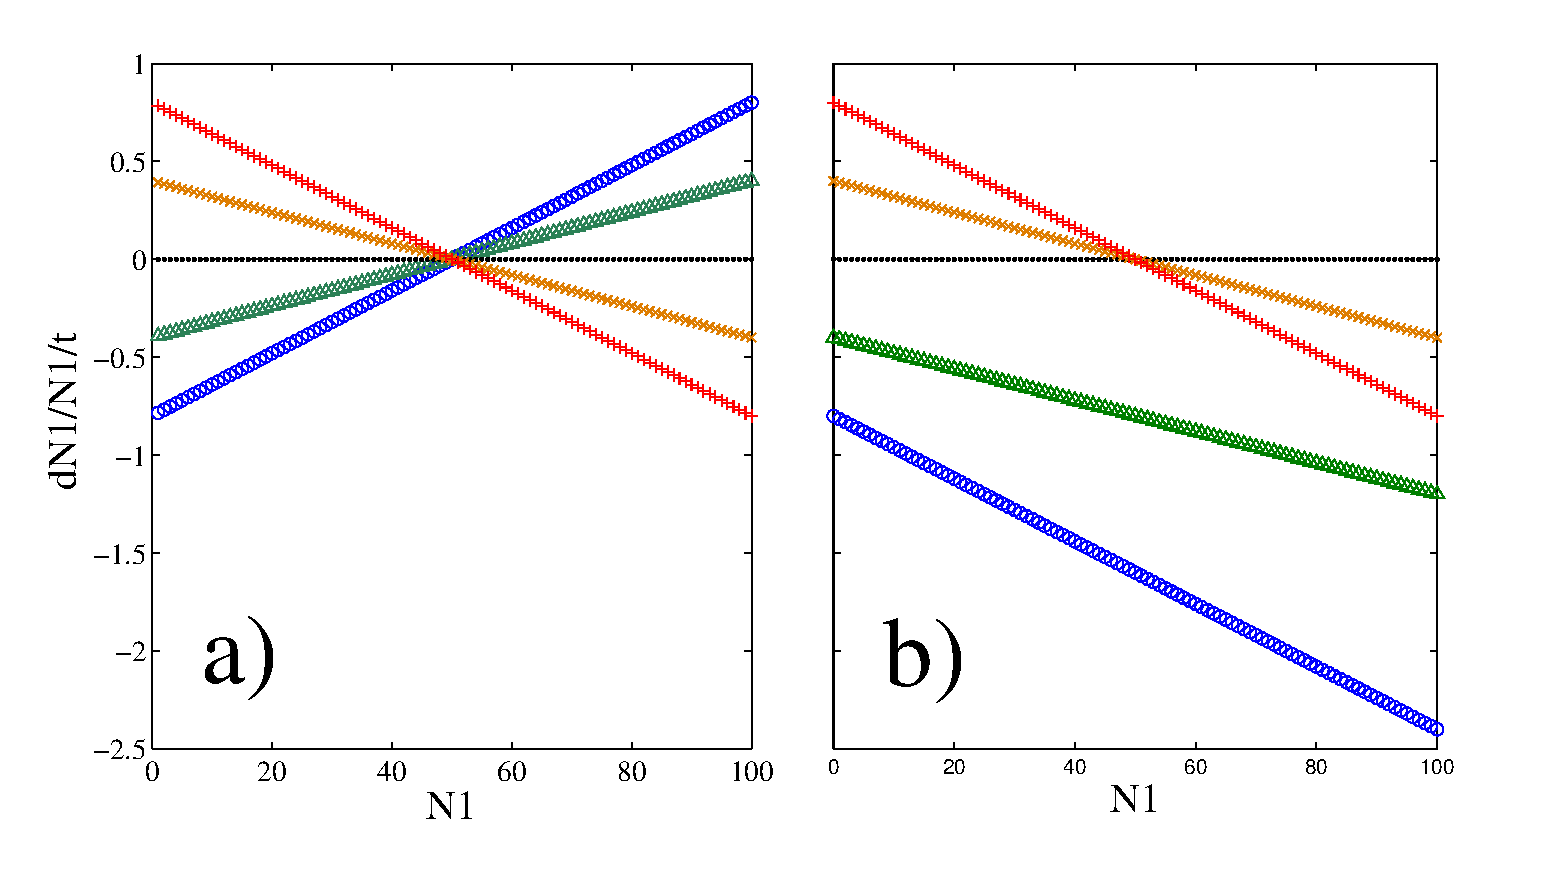
\includegraphics[scale=0.5]{DINAMICA_r1_Verh+modif_r1-p8p8K50.eps}
\caption{a) Tasas de crecimiento per cápita para la ecuación logística en la fórmula de Pearl, para las tasas vegetativas $r=-0.8$ (negro)
$r=-0.4$ (rojo), $r=0.4$ azul y $r=0.8$ naranja. b) La misma gráfica para la ecuación modificada de nuestro modelo.}
\label{fig:r_equiv_Verh+modif}
\end{figure}

Por su parte, la figura \ref{fig:r_equiv_Verh+modif}b muestra la tasa de crecimiento para nuestra fórmula modificada. En este caso la tasa per cápita dsiminuye siempre con el aumento de la población. Basados en esta idea proponemos un modelo de dinámica con capacidad de carga constante.

En el modelo de May se asume que la capacidad de carga y la tasa de crecimiento intrínseca de las especies son constantes e independientes del término mutualista. El efecto del mutualismo es un incremento de la tasa de crecimiento efectiva.

Para el sistema más simple posible, con una especie de cada clase, reescribimos el modelo de May:

\begin{align*}
\displaystyle & \frac{dN_1}{dt}= N_1 \, r_1\, \left(1 + \beta_{12}\frac{N_2}{K_1} \right) \, \left(1-\frac{N_1}{K_1}\right) \\
\displaystyle & \frac{dN_2}{dt}=N_2 \, r_2\, \left(1 + \beta_{21}\frac{N_1}{K_2} \right) \, \left(1-\frac{N_2}{K_2}\right)
\stepcounter{equation}\tag{\theequation}
\label{myeq3}
\end{align*}

El término dentro del primer paréntesis es un factor multiplicativo, siempre positivo y mayor que $1$, de la tasa vegetativa.
Ahora podemos reescribir las \textit{tasas de crecimiento equivalentes} como:

\begin{align*}
\displaystyle r_{\rm{eq},1}=r_1 + r_1\, \beta_{12} \frac{N_2}{K_1}\, =\, r_1 + b_{12}N_2  \\
\displaystyle r_{\rm{eq},2}=r_2 + r_2\, \beta_{21} \frac{N_1}{K_2}\, =\, r_2 + b_{21}N_1 \stepcounter{equation}
\tag{\theequation}
\end{align*}

Y con esta definición podemos reescribir:

\begin{align*}
\displaystyle & \frac{dN_1}{dt}= (r_1 + b_{12}\, N_2) \, N_1\,\left(1-\frac{N_1}{K_1}\right)=r_{\rm{eq},1}\,N_1\,\left(1-\frac{N_1}{K_1}\right) \\
\displaystyle & \frac{dN_2}{dt}= (r_2 + b_{21}\, N_1) \, N_2\,\left(1-\frac{N_2}{K_2}\right)=r_{\rm{eq},2}\,N_2\,\left(1-\frac{N_2}{K_2}\right)
\stepcounter{equation}\tag{\theequation}
\label{eq:May_reff}
\end{align*}

En ausencia de mutualismo se convierte en la ecuación logística modificada. El factor $\left(1-\frac{N_{1}}{K_{1}}\right)$ limita el crecimiento de la especie $1$ a la capacidad de carga $K_{1}$, y lo mismo sucede con la especie $2$, sin importar cual es la intensidad del mutualismo.

\begin{figure}[t]
\centering
%\includegraphics[scale=0.28]{rectas_optionI_2.eps}
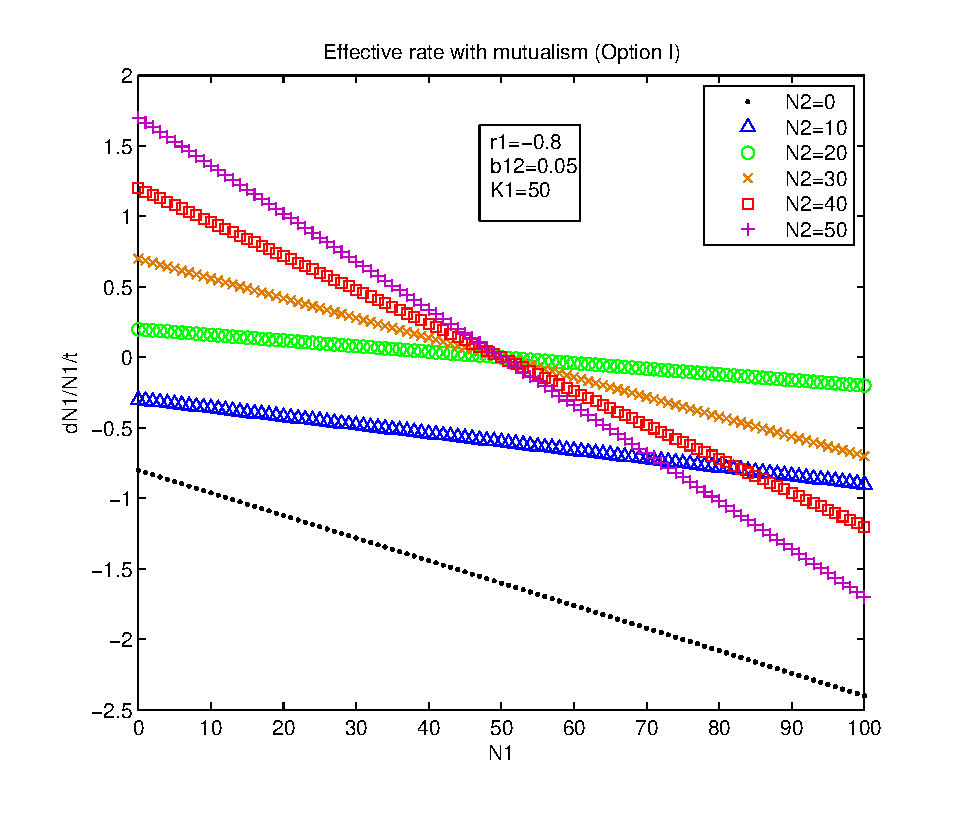
\includegraphics[scale=0.5]{DINAMICA_r1_eq_N1N2_r1p8b12p05K50.eps}
\caption{Per capita growth rate for species 1 with vegetative rate $r_1=-0.8$, carrying capacity $K_1=50$, and mutualism interaction coefficient $b_{12}=0.05$, for different values of population $N_2=0,10,20,30,40,50$.}
\label{fig:per capita_growth_rate_mutualism}
\end{figure}

Incluyendo la modificación usada en las ecuaciones \ref{eq:May_reff}, el modelo se puede escribir como:
\begin{align*}
\displaystyle & \frac{dN_1}{dt}= N_{1} \left( r_{\rm{eq},1}- |r_{\rm{eq},1}| \frac{N_1}{K_1} \right) = r_{\rm{eq},1}\, N_1 \left(1-sgn(r_{\rm{eq},1})\frac{N_1}{K_1}\right)\\
\displaystyle & \frac{dN_2}{dt}= N_{2} \left( r_{\rm{eq},2}- |r_{\rm{eq},2}| \frac{N_2}{K_2} \right)= r_{\rm{eq},2}\, N_2 \left(1-sgn(r_{\rm{eq},2})\frac{N_2}{K_2}\right)
\stepcounter{equation}\tag{\theequation}\label{eq:new_model}
\end{align*}

Como ya se ha indicado, la función $sgn(r_{\rm{eq}})$ tiene sentido biológico porque la competencia intra especie debe ser siempre negativa, con independencia del signo de la tasa vegetativa.

Para llegar a la fórmula general, generalizamos a una comunidad con $n$ esoecies de la clase $P$ (plantas), y $m$ especies de la otra $A$ (animales), que se relacionan por medio de una red de interacciones bipartita, pesada y bidireccional. Tomemos una especie $i$ de $P$ de población $N_i$ y otra $j$ de $A$ con $N_j$ individuos. Los pesos de la red representan la tasa de beneficio que recibe la población $i$ por la existencia de $j$. 

Las expresiones de las tasas de crecimiento de las especies $i$, $j$ quedan:
\begin{align*}
\displaystyle & r_{\rm{eq},i}  = \left( r_{b\, i} - r_{d\, i} \right) + \sum\limits_{k=1}^{m} b_{ik}\, N_k  \\
\displaystyle & r_{\rm{eq},j}  = \left( r_{b\, j} - r_{d\, j} \right) + \sum\limits_{l=1}^{n} b_{jl}\, N_l
\stepcounter{equation}\tag{\theequation}\label{modelors}
\end{align*}

Y el modelo con capacidades de carga constantes queda así:

\begin{theo}
\begin{align*}
\displaystyle
&\frac{dN_i}{dt}=r_{\rm{eq},i}\, N_i - |r_{\rm{eq},i}| \, \frac{{N_i}^2}{K_i}  \\
\displaystyle
&\frac{dN_j}{dt}=r_{\rm{eq},j} \, N_j - |r_{\rm{eq},j}| \, \frac{{N_j}^2}{K_j}
\stepcounter{equation}\tag{\theequation}\label{modelo_optionI}
\end{align*}
\end{theo}

\noindent donde en el subíndice $i$ corresponde a las especies de la clase $P$ y $j$ a las de la clase $A$. El término $r_{\rm{eq},i} - |r_{\rm{eq},i}| \frac{N_i}{K_i}$ es la tasa de crecimiento eficaz de la especie $i$, incluyendo los efectos del mutualismo y de la competencia intra especie. La figura \ref{fig:per capita_growth_rate_mutualism} es la tasa per cápita de la especie $1$ (en un sistema mutualista de $1+1$ especies),
con tasa vegetativa negativa $r_1=-0.8$ y coeficientes mutualistas $b_{12}=0.05$ y $K_1=50$, para los siguiente valores de población de la especie$N_2=0,10,20,30,40,50$. Para $N_2=20$, la tasa eficaz es todavía negativa, lo que conduciría a la destrucción del sistema. Para
$N_2=30$ la tasa ya es positiva y el sistema alcanzaría el máximo vital con las poblaciones en $K1$ y $K2$.

\subsection{Análisis de estabilidad para dos especies}

Las ecuaciones del sistema más simple, compuesto por una especia de planta a la que llamamos $1$ y una especia animal a la que llamamos $2$ son:
\begin{align*}
\displaystyle \frac{dN_1}{dt}= N_1 \left( r_{\rm{eff},1} - |r_{\rm{eff},1}| \frac{N_1}{K_1} \right) \\
\displaystyle \frac{dN_2}{dt}= N_2 \left( r_{\rm{eff},2} - |r_{\rm{eff},2}| \frac{N_2}{K_2} \right)
\stepcounter{equation}\tag{\theequation}\label{eq:two_species_model}
\end{align*}

\noindent donde $K_1$ and $K_2$ son las capacidades de carga. Las tasas de crecimiento efectivas son:
\begin{align*}
\displaystyle &r_{\rm{eff},1} = r_{1} + b_{12}\, N_2 \\
\displaystyle &r_{\rm{ef},2} = r_{2} + b_{21}\, N_1
\stepcounter{equation}\tag{\theequation}\label{eq:two_species_reff}
\end{align*}

En el sistema \ref{eq:two_species_model} se pueden idefnticar cinco puntos fijos:
la destrucción totoal ($N_1=0$,$N_2=0$), con independencia del valor de $r_{1}$ y $r_{2}$;
el máximo vital ($N_1=K_1$,$N_2=K_2$) que aparece si $r_{2}>0$ y $r_{1}>0$ simultáneamente (porque $b_{12}$ y $b_{21}$ son siempre positivos), es decir, cuando el mutualismo es facultativo para ambas especies; y las extinciones parciales, ($N_1=0$,$N_2=K_2$)
y ($N_1=K_1$,$N_2=0$) cuando $r_{2}>0$ y $r_{1}>0$ respectivamente, cuando el mutualismo es facultativo para una sola de las especies. Estas cuatro soluciones son equivalentes a las que aparecen en el modelo clásico de Verhulst. El quinto punto, y el más interesante para el análisis, aparece cuando el mutualismo es obligado para las dos especies, $r_{2}<0$ y $r_{1}<0$, y cuando $r_{\rm{ef},1}=r_{\rm{ef},2}=0$. Se corresponde con los valores de población ($N_1={-r_{2}}/{b_{21}}$, $N_2={-r_{1}}/{b_{12}}$).

El análisis de estabilidad lineal de los primeros cuatro puntos se puede hacer con el jacobiano, definido a partir de las ecuaciones de la dinámica de poblaciones
\begin{align*}
 \frac{dN_1}{dt} = f_1(N_1,N_2) \\
 \frac{dN_2}{dt} = f_2(N_1,N_2)
\stepcounter{equation}\tag{\theequation}\label{eq:Jacob00}
\end{align*}

\noindent como
\begin{equation}
%\begin{align*}
\mathbf{J}_{\left(N^{*}_1,N^{*}_2\right)}= \left.\left(
  \begin{array}{cc}
    \frac{\partial f_1}{\partial N_1} \, & \frac{\partial f_1}{\partial N_2}\\
    \\
        \frac{\partial f_2}{\partial N_1} \,& \frac{\partial f_2}{\partial N_2}
    \end{array} \right)\right|_{N^{*}_1,N^{*}_2}
\stepcounter{equation}\tag{\theequation}\label{eq:Jacob00}
%\end{align*}
\end{equation}

Para la solución trivial (extinción completa) el jacobiano es:
\begin{equation}
%\begin{align*}
\mathbf{J}_{\left(0,0\right)}= \left(
  \begin{array}{cc}
    r_1 & 0\\
    0 & r_2
    \end{array} \right)
\stepcounter{equation}\tag{\theequation}\label{eq:Jacob00}
%\end{align*}
\end{equation}

En la extinción total las tasas de crecimiento vegetativas $r_1$ y $r_2$, son los autovalores. En consecuencia, es una solución estable solo para el mutualismo obligado ( $r_{1}<0$ and $r_{2}<0$) e inestable en otro caso.

En $(0,K_2)$ el jacobiano vale:
\begin{equation}
%\begin{align*}
\mathbf{J}_{\left(0,K_2\right)}= \left(
  \begin{array}{cc}
    r_1+b_{12}K_2 & 0\\
    0 & -r_2
    \end{array} \right)
\stepcounter{equation}\tag{\theequation}\label{eq:Jacob0K2}
%\end{align*}
\end{equation}

Los dos autovalores son $\lambda_1=r_{1}+b_{12}K_2<0$ y $\lambda_2=- r_{2}$. La condición de estabilidad ($\lambda_{1}<0$ y $\lambda_{2}<0$) requiere $r_{2} > 0$ y $r_{1}<-b_{12}K_{2}<0$. Resultados equivalentes se obtienen para el punto $(K_1,0)$, bajo las condiciones $r_{1} > 0$ y $r_{2}<-b_{21}K_{1}<0$.

El jacobiano en la solución $(K_1,K_2)$ es: 
\begin{equation}
\mathbf{J}_{\left(K_1,K_2\right)}= \left(
  \begin{array}{cc}
    -r_1-b_{12}K_2 & 0\\
    0 & -r_2-b_{21}K_1
    \end{array} \right)
\stepcounter{equation}\tag{\theequation}\label{eq:JacobK1K2}
\end{equation}

Y hay un solo punto fijo estable cuando se dan las siguientes condiciones:
\begin{align*}
\displaystyle r^{\ast}_{\rm{ef},1} = r_{1} + b_{12}\, K_2 > 0 \\
\displaystyle r^{\ast}_{\rm{ef},2} = r_{2} + b_{21}\, K_1 > 0
\stepcounter{equation}\tag{\theequation}\label{eq:conditio2}
\end{align*}

Cuando ambas tasas efectivas de crecimiento son positivas, ambas poblaciones alcanzan las respectivas capacidades de carga.

El último punto fijo $({-r_{2}}/{b_{21}}, {-r_{1}}/{b_{12}})$ staisface que $r_{\rm{ef},1}=0$ y $r_{\rm{ef},2}=0$, y solo aparece para $r_{1}<0$ y $r_{2}<0$. En este caso el jacobiano no está definido porque la función valor anosluto no es diferenciable en $x=0$. Sin embargo, se puede estudiar la estabilidad en su vecindad bajo dos hipótesis, cuando $r_{\rm{ef}}>0$ y cuando $r_{\rm{ef}}<0$.

Podemos definir cuatro jacobianos dependiendo del signo de $r_{\rm{ef},1}$ y $r_{\rm{ef},2}$. En la vecindad de dicho punto las derivadas son:
\begin{align*}
\displaystyle \frac{\partial f_1}{\partial N_2} = -\frac{b_{12}}{b_{21}}r_2\left(1-sgn(r_{\rm{ef},1})\frac{r_2}{b_{21}K_1} \right)\\
\displaystyle \frac{\partial f_2}{\partial N_1} = -\frac{b_{21}}{b_{12}}r_1\left(1-sgn(r_{\rm{ef},2})\frac{r_1}{b_{12}K_2} \right)
\stepcounter{equation}\tag{\theequation}\label{eq:deriv_reff_0}
\end{align*}

Así, por ejemplo el jacobiano $\mathbf{J}^{+-}$ con $sgn(r_{eff},1)=+1$ y $sgn(r_{eff},\break2)=-1$ es
\begin{equation}
\mathbf{J}^{+-}= \left(
  \begin{array}{cc}
    0 & -\frac{b_{12}}{b_{21}}r_2\left(1-\frac{r_2}{b_{21}K_1} \right)\\
    -\frac{b_{21}}{b_{12}}r_1\left(1+\frac{r_1}{b_{12}K_2} \right)  & 0
    \end{array} \right)
\stepcounter{equation}\tag{\theequation}\label{eq:Jacob+-}
\vspace*{5mm}
\end{equation}

Los autovalores obtenidos de $\left| \mathbf{J}^{\pm,\mp}-\lambda\mathbb{I}  \right|=0$ son
\begin{align*}
  \lambda^{\pm,\mp}_{1,2}= \pm \sqrt{r_1 r_2 \left(1\pm\frac{r_2}{b_{21}}K_1 \right)\left(1\mp\frac{r_1}{b_{12}}K_2 \right)}
\end{align*}

Para cualquier definición de $sgn(r_{eff},1)$ y $sgn(r_{eff},2)$ todos los factores dentro de la raíz cuadrada son positivos, por tanto siempre hay un autovaloe positivo y otro negativo. Esto significa que en la vecindad del punto bajo estudio existe una cuenca de atracción y una de repulsión y por tanto es un \textit{saddle}.

Pese a que el jacobiano no está definico en este punto fijo, el diagrama de flujo puede obtenerse y solo una línea pasa por cualquier punto.

Este \textit{saddle} marca la frontera entre la cuenca de atracción de los otros puntos fijos estables y, en consecuencia, controla la resistenca del sistema ante perturbaciones externas. Si está próximo a la destrucción completa ($N_1=0$,$N_2=0$), el sistema es más estable porque la cuenca de atracción de $(K_1,K_2)$ es más extensa. Sucede lo contrario cuando se localiza cerca del máximo vital, con ambas poblaciones en capacidades de carga.

La figura \ref{fig:stab1_phase}a muestra las soluciones del sistema \ref{eq:new_model} para dos especies con mutualismo obligado ($r_1<0$ and $r_2<0$), e incio de las trayectorias en los puntos de la rejilla entre $10$ y $70$; la \ref{fig:stab1_phase}b es el diagrama de flujo en torno al \textit{saddle} en ($30,30$). Cuanto mayor sea la intensidad del mutualismo, más próximo se encuentra este punto al origen.

\begin{figure}
\centering
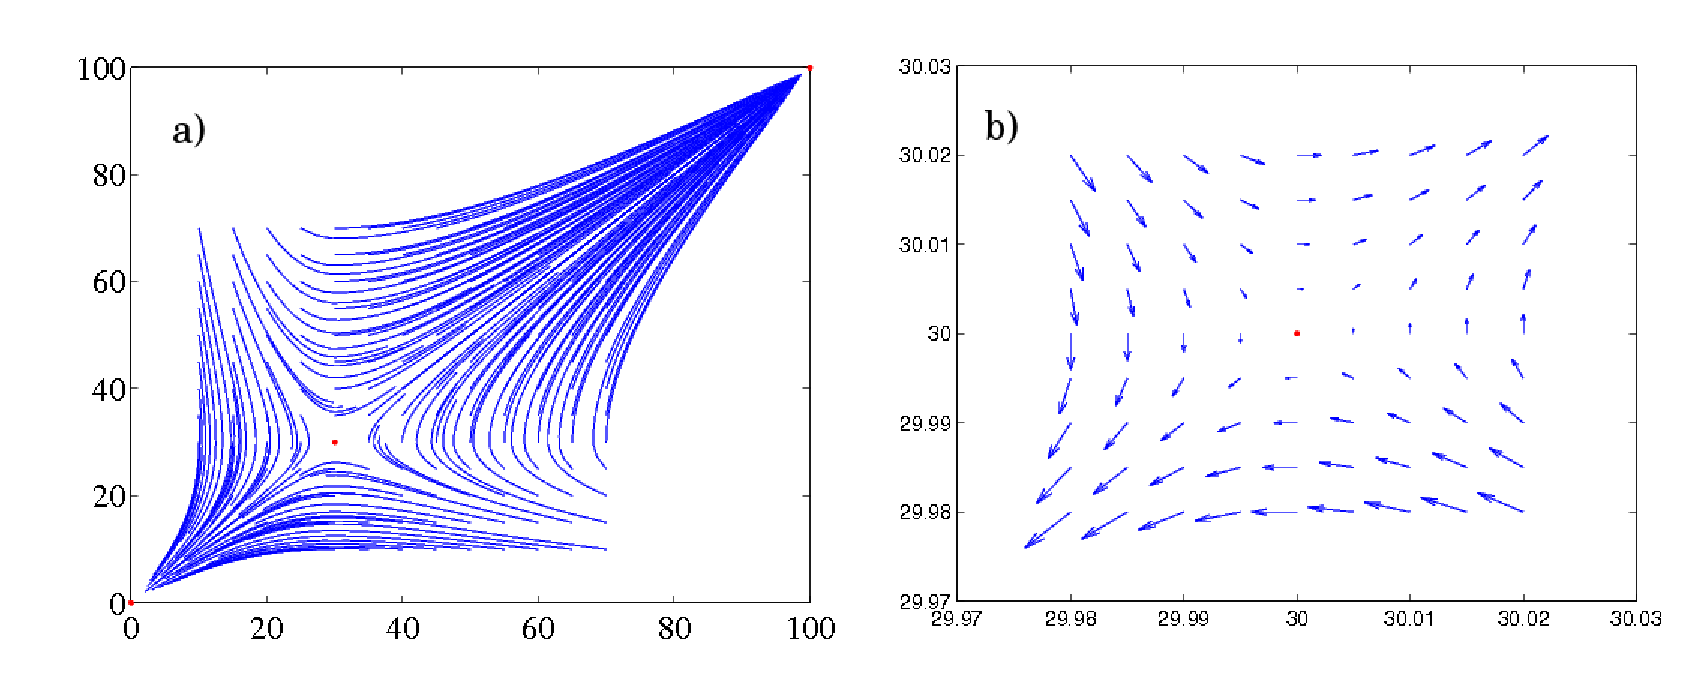
\includegraphics[scale = 0.5]{DINAMICA_solut_r9b03K100+flowdiagram.eps}
\caption {a) Soluciones del sistema \ref{eq:new_model} apara $r_1=r_2=-0.9$, $b_{12}=b_{21}=0.03$ y $K_1=K_2=100$. b) Diagrama de flujo en la vecindad del \textit{saddle} en ($30,30$). En rojo, los puntos fijos.}
\label{fig:stab1_phase}
\end{figure}

\subsection{Generalización con $n$ especies}

Para una red con múltiples especies, hay que analizar el sistema de ecuaciones \ref{modelo_optionI}. Los puntos fijos son, de nuevo, la extinción total ($N_i=0$, for all $i$), el máximo vital con todas las especies en sus capacidades de carga respectivas ($N_i=K_i$, for all $i$), y cualquier combinación de la solución trivial $N_{i}=0$ con las $N_{j}= K_{j}$, con la condición para las especies supervivientes:
\begin{equation}
\displaystyle r_{\rm{ef},j}^{\ast} = r_{j} + \sum_{l} b_{jl}\, K_{l} > 0 \\,
\label{eq:condit_reff_K}
\end{equation}

\noindent done $l$ es el índice para todas las especies de la clase diferentes de $j$ que alcanzan la capacidad de carga en el punto fijo ($N_{l}=K_{l}$).

El jacobiano para la extinción total es como la ecuación \ref{eq:Jacob00}, con las tasas vegetativas en la diagonal, y por tanto es una solución estable para mutualismo obligado ($r_i<0$ para todo $i$) e inestable en otro caso.

Para poblaciones en máximos, el jacobiano es como en \ref{eq:JacobK1K2}
\begin{equation}
%\begin{align*}
\displaystyle
\mathbf{J}_{\left(N_i=K_i, N_j=K_j\right)}= \left(
  \begin{array}{ccc}
    -r_{\rm{ef},i} & \cdots & 0\\
    \vdots & \ddots & \vdots \\
    0 & \cdots & -r_{\rm{ef},j}
    \end{array} \right)
\stepcounter{equation}\tag{\theequation}\label{eq:JacobK1K2}
%\end{align*}
\end{equation}

Esta solución es intrínsicamente estable porque todos los autovalores $\lambda_i=-r_{\rm{ef},i}^{\ast}$ son negativos (como en \ref{eq:condit_reff_K}).

La estabilidad de las soluciones de las extinciones parciales para $N_k=0$ y $N_l=K_l$, con
$k$ para las especies que se extinguen y $l$ para las que alcanzan sus capacidades de carga, puede deducirse de las entradas genéricas del jacobiano:
\begin{align*}
\displaystyle &\frac{\partial f_i}{\partial N_i} = r_{\rm{ef},i}-2\left|r_{\rm{ef},i}\right| \frac{N_i}{K_i}\\
\displaystyle &\frac{\partial f_i}{\partial N_j} = N_i\,b_{ij}-sgn\left(r_{\rm{ef},i}\right)b_{ij}\frac{{N_i}^2}{K_j}
\stepcounter{equation}\tag{\theequation}\label{eq:partial_ij}
\end{align*}

El jacobiano es diagonal con los valores

\begin{equation}
%\begin{align*}
\displaystyle
\mathbf{J}_{\left(N_k=0,N_l=K_l\right)}= \left(
  \begin{array}{ccc}
    r_{\rm{ef},k} & \cdots & 0\\
    \vdots & \ddots & \vdots \\
    0 & \cdots & -r_{\rm{ef},l}
    \end{array} \right)
%\stepcounter{equation}\tag{\theequation}
\label{eq:Jacob0_iK_j}
%\end{align*}
\end{equation}

\noindent donde las $r_{\rm{ef},k}$ son positivas porque

\begin{equation}
%\begin{align*}
\displaystyle
\left.\frac{\partial f_k}{\partial N_k} \right|_{N_k=0} = r_k + \sum_{l}b_{kl}K_l\\
\label{eq:partial_N_0}
\end{equation}

\noindent y las $r_{\rm{ef},l}$ son negativas porque
\begin{equation}
%\begin{align*}
\displaystyle
\left.\frac{\partial f_l}{\partial N_l} \right|_{N_l=K_l} = r_{\rm{ef},l} - 2 \left| r_{\rm{ef},l} \right| \frac{K_l}{K_l} \\
\label{eq:partial_N_K}
\end{equation}
%\end{align*}

\noindent y $r_{\rm{ef},l}>0$.

Entonces, la condición para que la extinción parcial sea estable es $r_k<-\sum_{s}b_{ks}K_s$, esto es, la tasa intrínseca de crecimimento de las especies que se extinguen es más negativa que menos la contribución mutualista de las especies a las que se conecta y $r_l>-\sum_{s}b_{ls}K_s$, esto es, la tasa intrínseca de crecimiento de las especies supervivientes es mayor que menos la contribución mutualista de sus benefecatoras.

Otros puntos fijos se obtienen de la condición $r_{\rm{ef},i}=0$, para todo $i$. Como se comentó en el caso de $1+1$ especies, la función valor absoluto no es diferenciable en $x=0$. Sin embargo, podemos definir las derivadas en la vecindad del pungo (\ref{eq:deriv_reff_0}). Suponiendo que $r_{\rm{ef},i}>0$ los términos del jacobiano son:
\begin{align*}
\displaystyle
&\left.\frac{\partial f_i}{\partial N_i} \right|_{r_{\rm{ef},i}=0^{+}} =0\\
&\left.\frac{\partial f_i}{\partial N_j} \right|_{r_{\rm{ef},i}=0^{+}} =N_i\,b_{ij} \left( 1- \frac{N_i}{K_i} \right) \equiv J_{ij}>0\\
\stepcounter{equation}\tag{\theequation}
\label{eq:partial_N_0}
%\end{equation}
\end{align*}

\noindent que es una matriz no negativa. Este punto fijo no es estable porque los autovalores no pueden ser simultáneamente negativos:
\begin{equation}
\displaystyle
  \sum_i \lambda_i = \rm{Tr} (\mathbf{J})
\end{equation}

Este es el punto intermedio de la solución, entre la extinción total y el máximo vital; si existe, es inestable.

\clearpage
\section{Modelo con saturación del beneficio}

La hipótesis de partida es que el mutualismo incrementa a tasa intrínseca de crecimiento de las especies. Esta suposición se basa en observaciones según las cuales la variación de la tasa de crecimiento de las poblaciones (o la fertilidad) tienen una alta correlación con la disponiblidad de recursos \cite{stenseth1998,krebs2002,rueness2003,tyler2008,jones2008}. En este contexto los recursos son las interacciones mutualistas. Supongamos que la comunidad está compuesta por $n_a$ especies de animales, con poblaciones$\{N_{i}^a\}$, y $n_p$ especies de plantas con poblaciones $\{N_{j}^p\}$. El beneficio mutualista entre las especies $i$  de una clase y $j$ de la otra se representa con el elemento $b_{ij}$ de la matriz de interacción. Debe tenerse en cuenta que las matrices no son necesariamente simétricas, y que la intensidad del beneficio de la interacción no es el mismo en ambos sentidos. Para una especie animal $i$, escribimos su tasa de de crecimiento como
\begin{align}
r_{i} = r_{i}^{0} + \sum_{k=1}^{n_{p}} b_{ik}\, N^{p}_k
\label{eq:expr}
\end{align}
En esta expresión, $r_{i}^{0}$ es la tasa de crecimiento vegetativo. Para impedir un crecimiento ilimitado de dicha tasa, el efecto del mutualismo tiene que saturar en cierto punto.

Siguiendo la idea de Velhurst, proponemos un modelo en el que el término de fricción $\alpha_i$ depende también de la intensidad de la interacción mutualista. La traducción biológica de esta idea es que a partir de un determinado nivel el aumento de individuos de la especie mutualista no aporta beneficio adicional. Imaginemos una especie de polinizadores y una planta de la que obtiene alimento en forma de néctar. Si la población de plantas crece sin medida, llegará un momento en que los insectos no podrán libar todo el néctar producido. Para mantener el modelo simple, suponemos que el efecto del mutualismo sobre $\alpha$ es proporcional al beneficio. 
\begin{align}
\alpha_i = \alpha_{i}^{0}+ c_{i} \sum_{k=1}^{n_{p}} b_{ik}\, N^{p}_k 
\stepcounter{equation}\tag{\theequation}
\label{eq:alphavariable}
\end{align}
El término $c_{i}$ es el coeficiente de proporcionalidad. Las expresiones para las plantas son similares con el sumatorio sobre las especies de animales. Para simplificar la notación, eliminaremos los ceros de $\alpha_{i}^{0}$ y $r_{i}^{0}$ allí donde no haya confusión posible. Bajo estas suposiciones la dinámica del modelo propuesto está gobernada por el siguiente juego de ecuaciones:

\begin{theo} 
Modelo de dinámica mutualista con saturación del beneficio.
\begin{align*}
\frac{1}{N^{a}_{i}}\frac{dN^{a}_{i}}{dt} = r_{i}+ \sum_{k=1}^{n_{p}} b_{ik}\, N^{p}_k - \left( \alpha_{i}+ c_{i} \sum_{k=1}^{n_{p}} b_{ik}\, N^{p}_k \right) N^{a}_{i} \nonumber\\
\frac{1}{N^{p}_{j}}\frac{dN^{p}_{j}}{dt} = r_{j}+ \sum_{\ell=1}^{n_{a}} b_{j\ell}\, N^{a}_\ell - \left( \alpha_{j}+ c_{j} \sum_{\ell=1}^{n_{a}} b_{j\ell}\, N^{a}_\ell \right) N^{p}_{j}
\stepcounter{equation}\tag{\theequation}\label{eq:DINAMICA_modeloralphaconmut}
\end{align*}
\end{theo}


Las expresiones en el lado derecho de las igualdades se pueden interpretar como \textit{tasas de crecimiento efectivas}. 

\begin{theo} 
Tasa de crecimiemto eficaz de la especie animal $i$.
\begin{equation}
r_{ef,i} = r_{i} + \sum_{k=1}^{n_{p}} b_{ik}\, N^{p}_k - \left( \alpha_{i}+ c_{i} \sum_{k=1}^{n_{p}} b_{ik}\, N^{p}_k \right) N^{a}_{i}
\label{eq:DINAMICA_effrate}
\end{equation}
\end{theo}

Las tasas efectivas de las especies de plantas se definen de forma similar sustituyendo $a$ por $p$. Las \textit{capacidades de carga} del sistema son los puntos fijos distintos de cero de las ecuaciones \ref{eq:DINAMICA_modeloralphaconmut}. Es sencillo ver que en ausencia de mutualismo $K_i = r_i/\alpha_i$ para la especie $i$. Por el contrario, en presencia de mutualismo muy intenso, $K_i$ tiende a $1/c_{i}$. El papel de la constante de proporcionalidad $c_i$ es, por tanto, limitar la población máxima de la especie $i$ cuando $c_{i} \sum_{k=1}^{n_p} b_{ik} \, N^p_{k} \gg \alpha_{i}$. 

Consideramos que este modelo podría resultar también válido para otro tipo de interacciones ecológicas en las que todos los términos $b_{ik}$ son positivos, como el comensalismo Commensalism ($b_{ij}=0, b_{ji}>0)$ y el antagonismo ($b_{mn}>0,b_{nm}<0$). 

\subsection{Análisis de estabilidad para dos especies}

Por simplicidad empezamos con la comunidad mutualista más sencilla, formada por una especie de cada clase, para la cual podemos obtener resultados análiticos completos. Sea la planta la especie que designamos con el índice $1$ y el animal la representada como $2$. El modelo \ref{eq:DINAMICA_modeloralphaconmut} se reduce a:

\begin{align}
\frac{dN^p_{1}}{dt} = \left( r_{1}+ b_{12}\, N^a_{2}\right) \ N^p_{1} - \left(\alpha_{1}+ c_{1} \, b_{12} \, N^a_{2} \right) {N^p_{1}}^2 ,\nonumber\\ 
\frac{dN^a_{2}}{dt} = \left( r_{2}+ b_{21}\, N^p_{1}\right)N^a_{2} - \left(\alpha_{2}+ c_{2} \, b_{21}\, N^p_{1} \right) {N^a_{2}}^2 .
\stepcounter{equation}\tag{\theequation}\label{eq:DINAMICA_dos_especies}
\end{align}

La figura \ref{DINAMICA_diagram} representa varios diagramas de flujo del sistema con distintas configuraciones de los parámetros.

\begin{figure*}
\centering
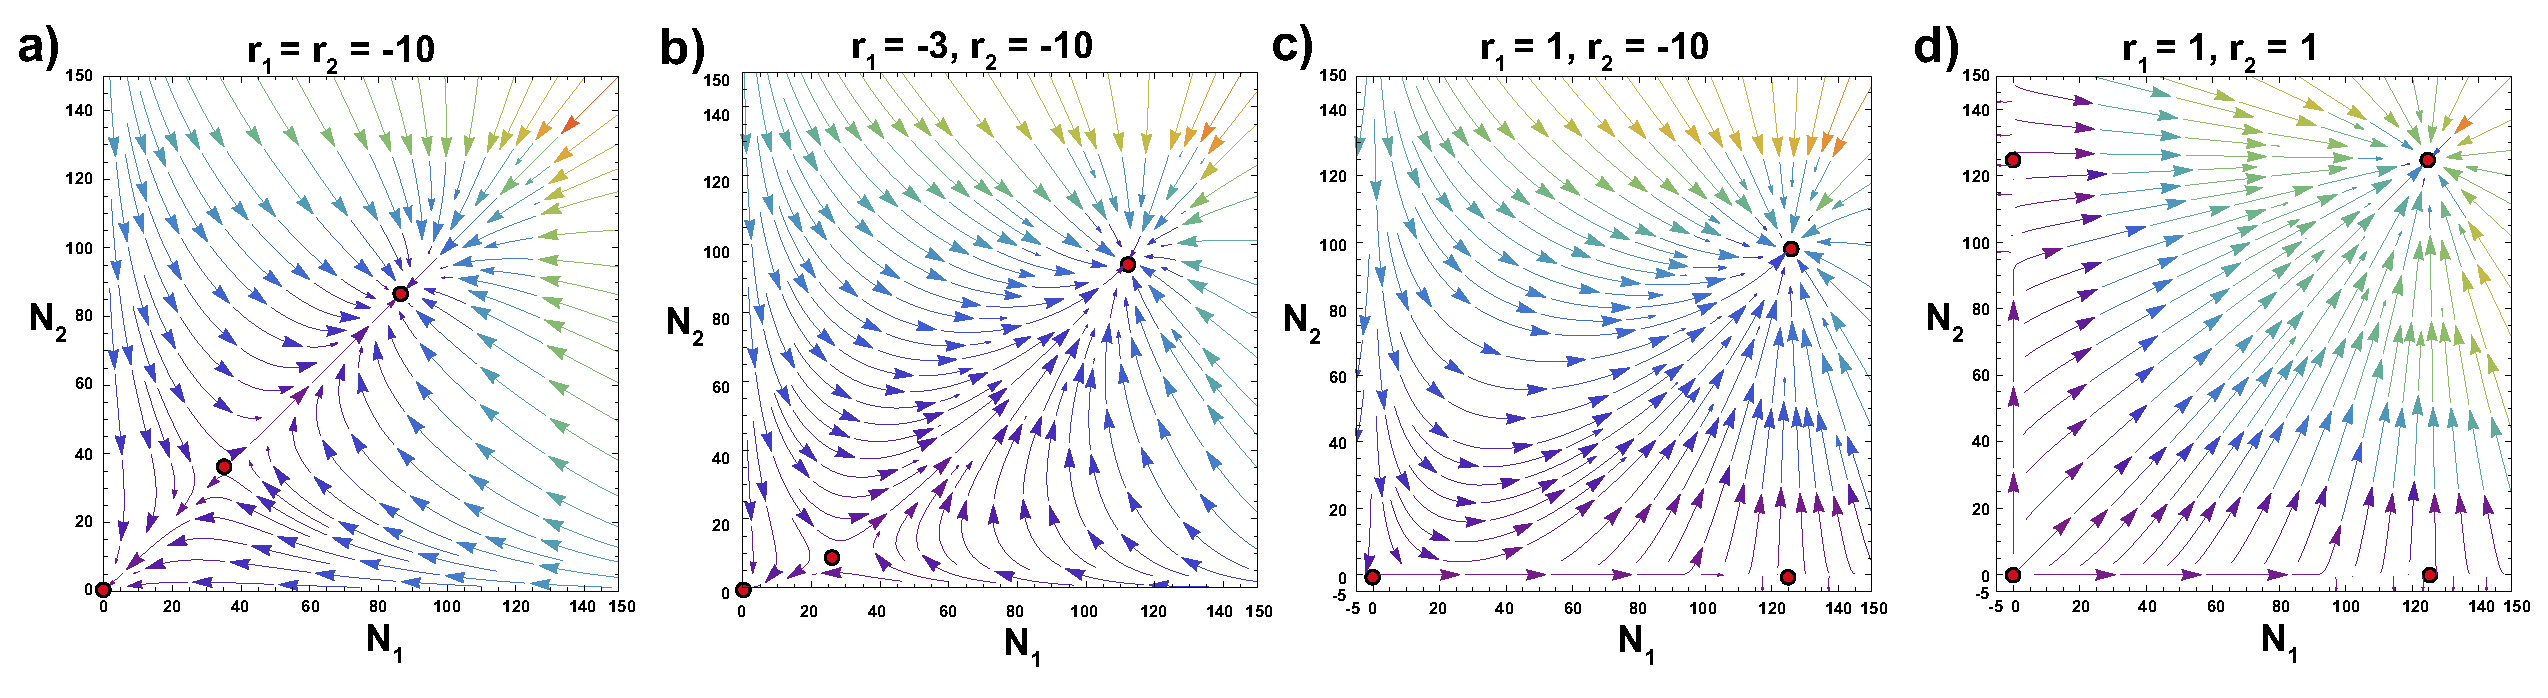
\includegraphics[scale=0.35]{DINAMICA_Figure1h.eps}
\caption {Diagrma de flujo de la dinámica de una comunidad de dos especies según el modelo de ecuaciones \ref{eq:DINAMICA_dos_especies}. Los puntos fijos se han resaltado como círculos de color rojo. El color de las flechas indica la intensidad del flujo. Las cuatro imágenes corresponden a diferentes valores para las tases intrínsecas de crecimimento. El resto de parámetros mantiene los mismos valores en los cuatro casos: $\alpha_1 = \alpha_2 = 0.008$, $b_{12} = b_{21} = 0.4$ and $c_1 = c_2 = 0.008$. El mutualismo es obligatorio en a) y b), aunque en diferente grado en el segundo diagrama. Es obligatorio para la especie 2 es c), mientras que la especie 1 podría sobrevivir sin la 2. En d) el mutualismo es facultativo para ambas especies.}
\label{DINAMICA_diagram}
\end{figure*}

Para encontrar los puntos fijos del sistema hacemos $\frac{dN^p_{1}}{dt} = \frac{dN^a_{2}}{dt} = 0$. El primero y más obvio, corresponde a la extinción total $({N^p_{1}}^*,{N^a_{2}}^*) = (0,0)$ con independencia del valor de los parámetros. Si cualquiera de las tasas de crecimiento intrínseco $r_1$, $r_2$ es positiva, entonces encontramos puntos fijos adicionales que aparecen por extinciones parciales. La dinámica de la población superviviente, con $r$ positivo, sigue en tal caso una ecuación logística como se deduce de la expresión \ref{eq:DINAMICA_dos_especies}. En consecuencia, su población tenderá a la capacidad de carga sin mutualismo ya sea $K_1 = r_1/\alpha_1$ o $K_2 = r_2/\alpha_2$. Las extinciones se producen en los puntos fijos $(K_1,0)$ o $(0,K_2)$, o en ambos si el mutualismo es facultativo solo para la especie $1$ ($r_1 >0$), solo para la especie dos $2$ ($r_2 >0$) (figura \ref{DINAMICA_diagram}c) o para las dos ($r_1>0$ y $r_2 >0$) (figura \ref{DINAMICA_diagram}d). 

Además de los puntos fijos correspondientes a extinciones, aparecen otros no triviales cuando se cumple la condición $r_{ef,i} = r_{ef,j} = 0$. Para dichos puntos se verifica que: 
\begin{align}
{N^p_{1}}^* = \frac{ r_{1}+ b_{12} \, {N^a_{2}}^* }{\alpha_{1}+ c_{1}\, b_{12}\, {N^a_{2}}^* } , \nonumber\\ 
{N^a_{2}}^* = \frac{ r_{2}+ b_{21}\, {N^p_{1}}^* }{\alpha_{2}+ c_{2} \, b_{21}\, {N^p_{1}}^* } .
\label{eq:DINAMICA_puntosfijos}
\end{align}

Sustituyendo la expresión de ${N^{a}_2}^*$ en la ecuación superior, encontramos que ${N^p_1}^*$ es la solución de una ecuación cuadrática en los puntos fijos: 
\begin{equation}
A\, {{N^p_1}^*}^2 + B \, {N^p_1}^* + C=0 ,
\label{eq:DINAMICA_quadra}
\end{equation}

Los coeficientes $A$, $B$ y $C$ valen:

\begin{align}
\displaystyle A &= c_{2}\, b_{21}\, \alpha_{1}+c_{1}\, b_{12}\, b_{21} , \nonumber \\
\displaystyle B &= \alpha_{1}\, \alpha_{2}+ c_{1}\, b_{12}\, r_{2} - c_{2}\, b_{21}\, r_{1} - b_{12}\, b_{21} ,\nonumber\\
\displaystyle C &= - r _{1}\, \alpha_{2} - b_{12}\, r_{2} .
\label{eq:DINAMICA_puntos_n1}
\end{align}

Los puntos fijos para ${N^a_2}^*$ se encuentran sustituyendo ${N^p_1}^*$ en la expresión inferior de la ecuación \ref{eq:DINAMICA_puntosfijos}. Aparecen distintos escenarios dependiendo de las soluciones de la ecuación \ref{eq:DINAMICA_quadra}:

\begin{enumerate}
\item Ambas raíces complejas. No hay puntos fijos que no supongan extinciones.
\item Una sola raíz real. Es un punto de bifuración de la dinámica del sistema. Las soluciones son reales pero degeneradas. En este caso existe un único punto fijo aparte de los de extinción. El estado final del sistema depende de la estabilidad de dicho punto. Sin embargo, lo más probable es que las poblaciones terminen extinguiéndose.
\item Dos raíces reales. La situación es similar a la representada en la imagen de la izquierda de la figura \ref{DINAMICA_diagram}. Hay dos puntos fijos no triviales, típicamente uno estable y un \textit{saddle} sobre la divisoria de las dos cuencas de atracción. La posición de este segundo punto depende de la extensión de la cuenca de extinción y, por tanto, de la resistencia del sistema ante perturbaciones externas. Lo denominamos \textit{umbral de extinción} y su valor lo representamos como$({N_{1}^{p}}^\bullet,{N_{2}^{a}}^\bullet)$.
\end{enumerate}

Para estudiar la estabilidad lineal de los puntos fijos, expandimos las ecuaciones \ref{eq:DINAMICA_dos_especies} en serie de Taylor en torno a ellos y calculamos el jacobiano del sistema (ver los detalles en el anexo....). Si los autovalores son negativos, el punto fijo es estable. En caso contrario, puede ser un \textit{saddle} si uno es positivo y otro negativo o inestable si ambos son negativos. Comenzando por la extinción total, el jacobiano puede escribirse como: 
\begin{equation}
J = \left(
\begin{array}{ll}
r_{1}   & 0 \\
0 & r_{2} 
\end{array}
\right) .\stepcounter{equation}\tag{\theequation}\label{eq:J00}
\end{equation}

Lo autovalores son $\lambda_{1,2} = r_{1,2}$, lo que indica que el punto de extinción es linealmente estable bajo la hipótesis de que $r_{1}<0$ y $r_{2}<0$; es decir, ambas especies dependen del mutualismo para sobrevivir. La extinción total tiene una cuenca de atracción para los distintos valores de las poblaciones. Si el sistema entra en ella, el único destino posible es la destrucción de la comunidad.

Por el contrario, si el mutualismo es facultativo para una o ambas especies, la extinción total se convierte en un \textit{saddle} o en un punto inestable. No obstante, pueden aparecer otros dos puntos fijos correspondientes a extinciones parciales. En estas circunstancias, la condición de estabilidad para $(r_1/\alpha_1, 0)$ es que $r_{1}>0$ y $r_{2}<-b_{21}\, r_{1}/\alpha_{1}$. Análogamente, $(r_1/\alpha_1, 0)$ es estable si y solo si  $r_{2}>0$ y $r_{1}<-b_{12}\, r_{2}/\alpha_{2}$.
El mismo análisis para los restantes casos de puntos fijos no triviales se traduce en jacobiano:

\begin{equation}
J = \left(
\begin{array}{ll}
- {N^{p}_{1}}^* \, (\alpha_{1}+ c_{1}\, b_{12} \, {N^a_2}^* )  & {N_{1}^{p}}^* \, b_{12} \, (1 - c_{1}\, {N_{1}^{p}}^* ) \\
{N_{2}^{a}}^* \, b_{21}\, (1 - c_{2}\, {N_{2}^{a}}^* ) & - {N_{2}^{a}}^* \, (\alpha_{2}+ c_{2}\,b_{21}\,{N_{1}^{p}}^* )
\end{array}
\right)\stepcounter{equation}\tag{\theequation}\label{eq:J}
\end{equation}
Como los parámetros $c_{1}$ y $c_2$ son siempre positivos (recordemos que son el inverso del límite de población en presencia de un mutualismo muy intenso), y que todos los términos de $J$ tienen el signo mostrado en la ecuación \ref{eq:J}. Los elementos de la diagonal son negativos, mientras que el resto son siempre positivos (una configuración similar del jacobiano para modelos mutualistas aparece en \cite{goh1979}. Esto implica que los autovalores de $J$ son ambos reales y pueden ser los dos negativos (\textit{puntos fijos estables}) o uno positivo y otro negativo (\textit{saddle}). La condición para la existencia de este últimoes que el determinante del jacobiano en el \textit{imbral de extinción} sea negativo, $J_{11} \, J_{22} < J_{12}\, J_{21}$, que en función de ${N_{1}^{p}}^\bullet$ y ${N_{2}^{a}}^\bullet$ significa que:

\begin{equation}
1-c_{1}\, {N_{1}^{p}}^\bullet - c_{2}\, {N_{2}^{a}}^\bullet > 0 .
\end{equation}

Todos estos resultados para dos especies indican que el modelo presenta una dinámica muy rica. Pese a ello, es los suficientemente simple para entender bien los diferentes regímenes y donde se localizan en el espacio de configuración de los parámetros. En este sentido, soluciona algunas de las limitaciones del modelo tipo II. Por ejemplo, encontrar una configuración para dos especies como la que aparece en la figura \ref{DINAMICA_typeII} requiere un esfuerzo considerable de afinamiento de los pará,etros. Esta configuración con dos atractores y una divisoria nítida es ideal para estudiar fenómenos como la resistencia de la red, la capacidad de soportar una alta biodiversidad o la evolución de las interacciones de la red \cite{bastolla2009, suweis2013emergence}. Este régimen aparece de forma natural en el modelo propuesto, como se ve en la figura \ref{DINAMICA_diagram}, sin la necesidad de un complejo proceso de afinamiento. Además, como veremos en los siguientes apartados, una configuración equivalente con un atractor de extinción, otro con poblaciones finitas y una clara divisoria, aparece al extender el estudio a redes con muchas más
especies.

\begin{figure}
\centering
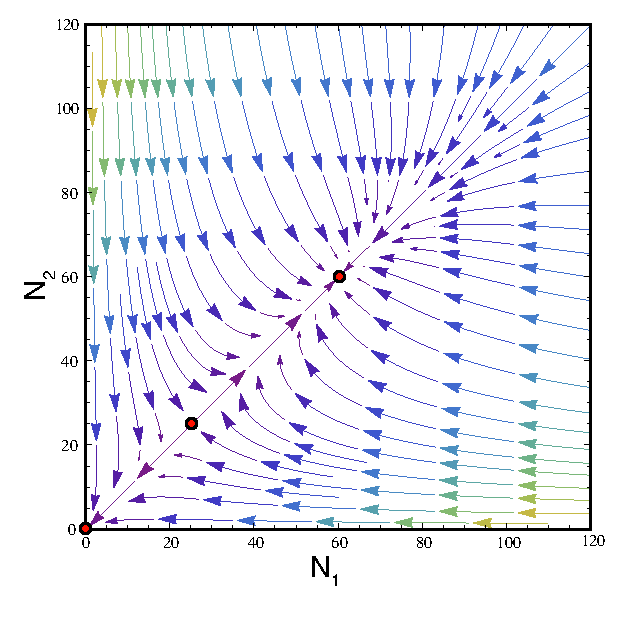
\includegraphics[scale=0.6]{DINAMICA_Figure2.eps}
\caption {Diagrama de flujo para la dinámica de ecuaciones de tipo II \ref{DINAMICA_eq_typeII}. Encontrar esta configuración requirió un ajuste de parámetros laborioso. Los valores empleados en este ejemplo son $r_1 = r_2 = -0.1$, $\alpha_1 = \alpha_2 = 0.001$, $a = 0.066$, $b = 0.2$ and $T_H = 1$.}
\label{DINAMICA_typeII}
\end{figure}

\subsection{La divisoria de la vida}
\label{watershed}

Llamaremos \textit{divisoria de la vida} al límte que separa las trayectorias que evolucionan hacia la capcidad máxima de población del sistema de las que terminan en su destrucción. En la imagen izquierda de la figura \ref{DINAMICA_diagram} es la curva que claramente delimita ambas cuencas. La divisoria incluye al \textit{saddle} no trivial $({N_1^p}^\bullet,{N_2^a}^\bullet)$, esto es la combinación mínima de poblaciones que garantiza la supervivencia. Su posición en el espacio de fases es importante porque determina la posición base de dicha curva y en consecuencia la fragilidad del sistema, que se expresa como la relación de áreas entre las dos cuencas de atracción. La distancia de este punto al máximo de poblaciones indica la resistencia ante perturbaciones externas. Si es muy pequeña, una ligera disminución del número de individuos, provocada por enfermedades, sequías o siniestros cualquier naturaleza puede llevar al sistema a la cuenca de destrucción. Por el contrario, si esta distancia es grande, la comunidad podrá recobrarse de estos eventos y crecer de nuevo hacia el máximo. Como los ciclos naturales suelen ser cíclicos, la combinación de poblaciones se moverá de manera habitual entre estos puntos, y un amplio rango dinámico facilita la permanencia en el tiempo. 

Para el sistema mínimo, de dos especies, las principales características de la divisoria se pueden encontrar analíticamente. Los puntos de la curva se corresponden a los pares de poblaciones $({N_1^p},{N_2^a})$ para los cuales la dinámica del sistema evoluciona exactamente sobre la curva y termina en el atractor $({N_1^p}^\bullet,{N_2^a}^\bullet)$. Sabemos que es un punto inestable y que la menor perturbación conducirá hacia uno u otro lado de la divisoria, pero conocer la expresión analítica de la curva supone un gran avance.  

Por definición, en $({N_1^p}^\bullet,{N_2^a}^\bullet)$ las tasas efectivas de crecimiento son nulas. Para llegar a este punto desde cualquier otro de la divisoria, las tasas de ambas especias deben ser de signo contrario y evolucionar en el tiempo de forma similar. Si las dos fueran del mismo signo, las trayetorias irían hacia la extinción (negativo) o hacia el máximo vital (positivo). 

Supongamos que el sistema se aproxima a $({N_1^p}^\bullet,{N_2^a}^\bullet)$, desde una posición inicial $({N_1^p}^0,{N_2^a}^0)$ pertencienta a la divisoria. Las tasas efectivas de crecimiento son:

\begin{align}
r_{ef,1}  = & \, A \, e^{-\gamma\, t} ,\nonumber\\  
r_{ef,2}  = & -B\, e^{-\gamma\, t} , 
\label{eq:coeffsreffs}
\end{align}
donde $A$, $B$ y $\gamma$ son constantes desconocidas por el momento. El sistema de ecuaciones \ref{eq:DINAMICA_dos_especies} se convierte en el siguiente:
\begin{align}
\frac{dN^p_{1}}{dt} & = N^p_{1} \, A \, e^{-\gamma \, t} , \nonumber \\
\frac{dN^a_{2}}{dt} & = -N^a_{2}\, B \, e^{-\gamma \, t} .
\label{eq:coeffsreffs_2}
\end{align}

Integrando ambas ecuaciones entre $t = 0$ e infinito  encontramos que:

\begin{align}
 \ln \frac{{N_1^p}^\bullet}{{N_{1}^p}^0} & = \frac{A}{\gamma} , \nonumber\\ 
 \ln \frac{{N_2^a}^\bullet}{{N_{2}^a}^0} & = - \frac{B}{\gamma} .
\label{eq:coeffsreffs_3}
\end{align}

Como el valor de $\gamma$ tiene que ser el mismo para ambas expresiones, obtenemos la condición que tienen que cumplir $({N_1^p}^0,{N_2^a}^0)$ para pertenecer a la divisoria:

\begin{align}
\frac{1}{B} \ln \left(\frac{{N_{2}^a}^\bullet}{{N_{2}^a}^0} \right) + \frac{1}{A} \ln \left(\frac{{N_1^p}^\bullet}{{N_1^p}^0} \right) = 0 ,
\label{eq:coeffsreffs_4}
\end{align}

Esto significa que la expresión funcional de la divisoria es una ley de potencia.

\begin{align}
{N_2^a}^0 = C\, ({N_1^p}^0)^\frac{-B}{A}. 
\label{eq:powerlaw}
\end{align}
Podemos despejar la constante $C$ teniendo en cuenta que la divisoria incluye el punto fijo $({N_1^p}^\bullet,{N_2^a}^\bullet)$, así que podemos escribir:

\begin{align}
C = {N_2^a}^\bullet / ({N_1^p}^\bullet)^\frac{-B}{A} .
\end{align}

Para encontrar el valor del exponente fraccionario $\frac{B}{A}$, debemos volver a la definición de ñas tasas de crecimiento efectivas $r_{ef,1}$ y $r_{ef,2}$. De acuerdo con las ecuaciones \eqref{eq:coeffsreffs}, en $t=0$ tenemos que:
 
\begin{align}
A = & \, r_{1}+ b_{12}\, {N_2^a}^0 - (\alpha_{1}+ c_{1} \, b_{12}\, {N_{2}^a}^0) \, {N_1^p}^0 , \nonumber\\
-B = &\, r_{2} + b_{21} \, {N_{1}^p}^0-(\alpha_{2}+ c_{2}\,  b_{21}\, {N_{1}^p}^0)\,  {N_{2}^a}^0 .
\label{eq:reffs_2especies}
\end{align}

Si sabemos que nuestro punto inicial era parte de la divisoria, podemos obtener el valor del exponente diviendo estas expresiones. Alternativamente, si necesitamos encontrar otros puntos de la divisoria que no sean $({N_1^p}^\bullet,{N_2^a}^\bullet)$, podemos dividir las expresiones anteriores y, usando la ecuación \ref{eq:coeffsreffs_3}, llegar a la siguiente ecuación implícita:

\begin{align}
\frac {\ln \left( \frac{{N_2^a}^\bullet}{{N_2^a}^0} \right)}{\ln \left( \frac{{N_1^p}^\bullet}{{N_1^p}^0} \right)} = \frac{( r_{2}+ b_{21}\, {N_1^p}^0) - (\alpha_{2}+ c_{2} \,  b_{21}\, {N_1^p}^0 ) \, {N_1^p}^0}{( r_{1}+ b_{12}\, {N_2^a}^0) - (\alpha_{1}+ c_{1} \, b_{12}\, {N_2^a}^0 ) \, {N_2^a}^0 } .
\label{eq:implicita_watershed}
\end{align}

Resolviendo esta ecuación de forma numérica podemos encontrar cualquier punto de la divisoria, y con ello obtenemos el valor del exponente $\frac{B}{A}$. La figura \ref{fig:powerlaw} muestra un ejemplo concreto de divisoria, y una comparación entre la curva definida por el sistema \ref{eq:powerlaw} y la ecuación implícita \eqref{eq:implicita_watershed}. Ambas se han resuelto por intergación numérica. Los puntos rojos se han encontrado haciendo un barrido del espacio de parámetros en una aproximación de \textit{fuerza bruta}, determinando el límite entre extinción y evolución hacia la capacidad máxima. La línea gris continua es la ley de potencia que se obtiene resolviendo las ecuaciones \eqref{eq:powerlaw} and \eqref{eq:implicita_watershed}

\begin{figure}[ht!]
\centering
\includegraphics[scale=0.5]{DINAMICA_Figure3.eps}
\caption {Divisoria de la vida para dos especies. En este caso, $\frac{B}{A}=1.2944,~{N_1^p}^\bullet=989,~{N_2^a}^\bullet=1232,~b_{12}=0.000041850,~c_{1}=0.00004,~\alpha_{1}=~0.000035,~r_1=-0.016,~b_{21}=0.00008750,~c_{2}=0.0001,~\alpha_{2}=0.000035,~r_2 =-0.02$.}
\label{fig:powerlaw}
\end{figure}

\subsection{Generalización con $n$ especies}
 
La generalización del análisis de establidad para un número cualquiera de especies es simple. Los puntos fijos del sistema \ref{eq:DINAMICA_modeloralphaconmut} incluyen la solución trivial de destrucción del sistema $(N_{i}^p,\cdots, N_{j}^a) = (0, \cdots,0)$, los puntos de extinción parcial cuando el mutualismo es facultativo para algunas especies y los puntos fijos no triviales $({N^{a}_{i}}^*,\cdots,{N^{p}_{j}}^*)$ en los que las tasas de crecimiento efectivas son nulas:
\begin{align}
r^{*}_{ef,i}  = (r_{i}+ \sum_{k=1}^{n_{p}}\,  b_{ik}\, {N^p_{k}}^*)- (\alpha_{i}+c_{i}\, \sum_{k=1}^{n_{p}} b_{ik}\, {N^{p}_k}^* )\, {N^{a}_{i}}^* = 0 \nonumber ,\\
r^{*}_{ef,j}  = (r_{j}+ \sum_{\ell=1}^{n_{a}} b_{j\ell}\, {N^{a}_{\ell}}^*)- (\alpha_{j}+c_{j}\, \sum_{\ell=1}^{n_{a}} b_{j\ell}\, {N^{a}_\ell}^* )\, {N^{p}_{j}}^* 
=0 ,
\label{eq:effrate2}
\end{align}
Estas son las expresiones para animales y plantas. Se puede reescribir el sistema como:

\begin{align}  
{N^{a}_{i}}^* = \frac{r_{i}+\sum_{k=1}^{n_{p}}b_{ik}\, {N^{p}_{k}}^*}{\alpha_{i}+c_{i}\,\sum_{k=1}^{n_{p}}{b_{ik}N^{p}_{k}}^*} = 
  \frac{r_{i}+r_{i}^{mut}}{\alpha_{i}+c_{i}\, r_{i}^{mut}} = 
  \frac{r_{i}^{*+}}{r_{i}^{*-}} , \nonumber\\
{N^{p}_{j}}^*=\frac{r_{j}+\sum_{\ell=1}^{n_{a}}b_{j\ell}\, {N^{a}_{\ell}}^*}{\alpha_{j}+c_{j}\,\sum_{\ell=1}^{n_{a}}{b_{j\ell}N^{a}_{\ell}}^*} =
  \frac{r_{j}+r_{j}^{mut}}{\alpha_{j}+c_{j}r_{j}^{mut}} =
  \frac{r_{j}^{*+}}{r_{j}^{*-}} .
\end{align}

Donde las tasas $r_{i}^{mut}$ representan el efecto del mutualismo sobre la especie $i$, mientras que las tasas $r^{*+}$ son las que incrementan el crecimento de la población y las $r^{*-}$ las que lo disminuyen vía competición intra especies. 

Las ecuaciones  \ref{eq:DINAMICA_modeloralphaconmut} se pueden linealizar en torno a los puntos fijos. El jacobiano correspondiente tiene el mismo aspecto que el correpondiente al sistema mínimo de dos especies (ecuación \eqref{eq:J}), con términos negativos en la diagonal de la matriz y positivos o nulos fuera de ella. Para los puntos fijos no triviales se pueden escribir como (véase el Anexo \ref{DINAMICA_ANEXO_estabilidad}):
\begin{align}
\displaystyle & J_{ii}= - {N^{a}_{i}}^* \left(\alpha_{i} + c_{i} \,  \sum_{k=1}^{n_{p}} b_{ik} {N^{p}_{k}}^* \right), \nonumber\\
\displaystyle & J_{jj}= - {N^{p}_{j}}^* \left(\alpha_{j} + c_{j} \, \sum_{\ell=1}^{n_{a}} b_{j\ell}\, {N^{a}_{\ell}}^*\right).
\label{eq:Jii}
\end{align}
Los coeficientes fuera de la diagonal son:
\begin{align}
\displaystyle & J_{ij}={N^{a}_{i}}^* \, b_{ij}\, \left( 1-c_{i}\, {N^{a}_{i}}^*\right) 
\label{eq:Jij1}
\end{align}
para la interacción entre una especie animal $i$ y una planta $j$, y 
\begin{align}
\displaystyle & J_{ji}={N^{p}_{j}}^* \, b_{ji}\, \left( 1-c_{j}\, {N^{p}_{j}}^*\right)
\label{eq:Jij2}
\end{align}
para la correspondiente al sentido planta $j$ y animal $i$. Dada la invariancia de la traza de la matriz bajo un cambio de la base vectorial, la suma de autovalores de la matriz debe satisfacer la siguiente relación:
\begin{equation}
  \sum_{k}^{n_{a}+n_{p}} \lambda_{k}= - \left(\sum_{k}^{n_{a}+n_{p}} |J_{kk}| \right) .
  \stepcounter{equation}\tag{\theequation}\label{eq:sum_lambdas2}
\end{equation}
La traza es negativa, lo que significa que si hay autovalores positivos o nulos su efecto debe compensarse por otros autovalores negativos. En consecuencia, los puntos fijos no triviales pueden ser estables si todos los autovalores son negativos, o \textit{saddle} si al menos uno de ellos en positivo. No es posible que sean puramente inestables.

Otro extremo que hay que investigar es lo que sucede en caso de extinciones parciales. El efecto de la desaparición de algunas especies es reducir las dimensiones del sistema de ecuaciones \ref{eq:DINAMICA_modeloralphaconmut}. Para hacerlo más simple, asumamos, por ejemplo, que la especie animal $e$ se extingue. Esto significa que los posibles puntos fijos del sistema deben incluir ahora ${N_e^a}^* = 0$. El colapso de $e$ puede provocar la extinción de algunas especies de plantas que se alimentaban con su polen, frutos o semillas, dependiendo del tipo de red. Estas extinciones pueden, a su vez, desencadenar la desaparición de especies animales que dependían de dichas plantas para su ciclo reproductivo. Este encadenamiento catastrófico es lo que se conoce como extinción en cascada. Aunque el fenómeno que produce la primera extinción sea externo y afecte a una sola especie, todas las demás se ven afectadas porque su dinámica está enlazada por el sistema de ecuaciones completo. Los nuevos puntos fijos no triviales se corresponden con los de extinción parcial del sistema original. La estabilidad de dichos puntos puede cambiar de manera sustancial con esta alteración de las condiciones. Los términos del jacobiano de las especies desaparecidas se convierten en $J_{ee} = r_e + \sum_{k =1}^{n_p }b_{ek}\,{N_k^p}^*$ en la diagonal y $J_{ej} = 0$ fuera de ella. Estos términos dejan de contribuir a los autovalores relevantes para la estabilidad del sistema. El resto de coeficientes del jacobiano se obtienen de las ecuaciones \ref{eq:Jii}, \ref{eq:Jij1}, y \ref{eq:Jij2} adaptadas a las especies supervivientes. Esto implica que los sumatorios de las ecuaciones \eqref{eq:Jii} ya no incluyen todas las especies y que los términos de la diagonal pueden estar más próximos a cero. La establidad de los nuevos puntos fijos puede variar dependiendo de los parámetros de las ecuaciones del modelo de dinámica de poblaciones de las especies supervivientes. En realidad, dependiendo de la configuración resultante de la comunidad reducida, el sistema puede ser más robusto ante extinciones parciales que antes. Esto puede explicar por qué las comunidades mutualistas adoptan configuraciones fuertemente anidadas, son el resultado por prueba y error en el tiempo de extinciones parciales y de la llegada de nuevas especies que alteran su dinámica.   

\section{Material y métodos}

Para este capítulo hemos utilizado la cole....

\subsection{Integración de las ecuaciones}
\label{DINAMINCA_NumSim}

Los modelos de población manejan cantidades discretas y la simulación es una herramienta potente para manejar la dinámica y el comportamiento estocástico. La elección de un método específico de simulación depende de su precisión y eficacia computacional y a veces representa un desafío.

Por ejemplo, los modelos discretos de Markov se han utilizado con frecuencia para este tipo de simulaciones, pero esta estrategia tiene desventajas comparada con la simulación estocática discreta, ya sea basada en la distribución de Poisson o en la binomial. Para los modelos de Markov de dimensiones moderadas, el número de estados puede ser muy grande, minetras que las simulaciones basadas en Poisson o binomial, con su manejo de variables de estado agregadas es mucho más rápida  \cite{gustafsson2007bringing, balcan2009multiscale}.

Hemos elegido la simulación binomaial para resolver las ecuaciones de ambos modelos. Esta técnica es una extensión de la simulación de sistemas continuos y una elección razonable cuando el resultado del proceso aleatorio tiene solo dos posibles valores. Por ejemplo, la supervivencia en un intervalo finito de tiempo es un ensayo de Bernoulli, el individuo sobrevive o no. La reproducción también puede modelarse adecuadamente como un ensayo de Bernouilli si el intervalo de simulación es pequeño. 

Para una especie con una tasa intrínseca de crecimiento $r$, podemos suponer que la probabilidad de reproducción en un intervalo $\Delta T$ sigue una distribución exponencial de valor medio $1/r$. Así, la probabilidad de reproducción es:
\begin{equation}
\label{eq:probbreeding}
P = \int_0^{\Delta T} \! re^{-r\, t}  \, dt = 1 - e^{-r\, \Delta T}
\end{equation}
In particular, a population of $N$ individuals in time $t$, with pure exponential growth, will be in $t+\Delta T$:
\begin{equation}
N(t+\Delta T)=N(t) + sgn \left(r \right) Binomial \left( N(t),P \right)
\end{equation}
\noindent El sistema de ecuaciones toma la forma estocástica siguiente:
\begin{equation}
\begin{split}
N^{a}_{j}(t+\Delta T)=N^{a}_{j}(t) + sgn \left(\hat{r}^{a}_{ef,j} \right) Binomial \left( N^{a}_{j}(t),P^{a}_{j}\right)\\
N^{p}_{l}(t+\Delta T)=N^{p}_{l}(t) + sgn \left(\hat{r}^{p}_{ef,l} \right) Binomial \left(N^{p}_{l}(t),P^{p}_{l} \right)
\end{split}
\end{equation}
\noindent donde $\hat{r}^{a}_{ef,j}$ es la tasa de crecimiento efectiva de la especie $j$ de la clase $a$ durante el periodo de simulación, y $P^{a}_{j}, P^{p}_{l}$ , las probabilidades de crecimiento según la ecuación \ref{eq:probbreeding}. En particular, si se trabaja con intervalos de un día, como en nuestros experimentos:
\begin{equation}
\hat{r}_{ef} = (1+r_{ef})^{1/365}-1
\end{equation}

La simulación estocástica tiene una ventaja adicional de gran interés para nuestras simulaciones. Las perturbaciones externas se modelan como variaciones temporales de la tasa efectiva de reproducción, restando el efecto del siniestro. Computacionalmente es muy sencillo llevar a cabo esta modificación; si, por el contrario, se resuelven numéricamente las ecuaciones diferenciales, es necesario cambiar las condiciones iniciales para cada nueva perturbación y garantizar la continuidad en dichos puntos.

\section{Resultados}

Nunc posuere quam at lectus tristique eu ultrices augue venenatis. Vestibulum ante ipsum primis in faucibus orci luctus et ultrices posuere cubilia Curae; Aliquam erat volutpat. Vivamus sodales tortor eget quam adipiscing in vulputate ante ullamcorper. Sed eros ante, lacinia et sollicitudin et, aliquam sit amet augue. In hac habitasse platea dictumst.

\subsection{Simulaciones con capacidades de carga constantes}
\label{results_K_constante}
Es muy complicado obtener resultados analíticos para una comunidad mutualista por la compleja red de interacciones entre las especies \cite{bastolla05,bastolla09}. En este apartado se muestran los resultados de simulaciones numéricas que sirve para explorar la estabilidad de las soluciones del modelo \ref{modelo_optionI}. Se han simulado situaciones dentro de las tres cuencas de atracción, esto es, extinción total, extinciones parciales y supervivencia en capacidades de carga. Los parámetros de las simulaciones se listan en el Anexo \ref{DINAMICA_ANEXO_KConst}.

\begin{figure}[h!]
\centering
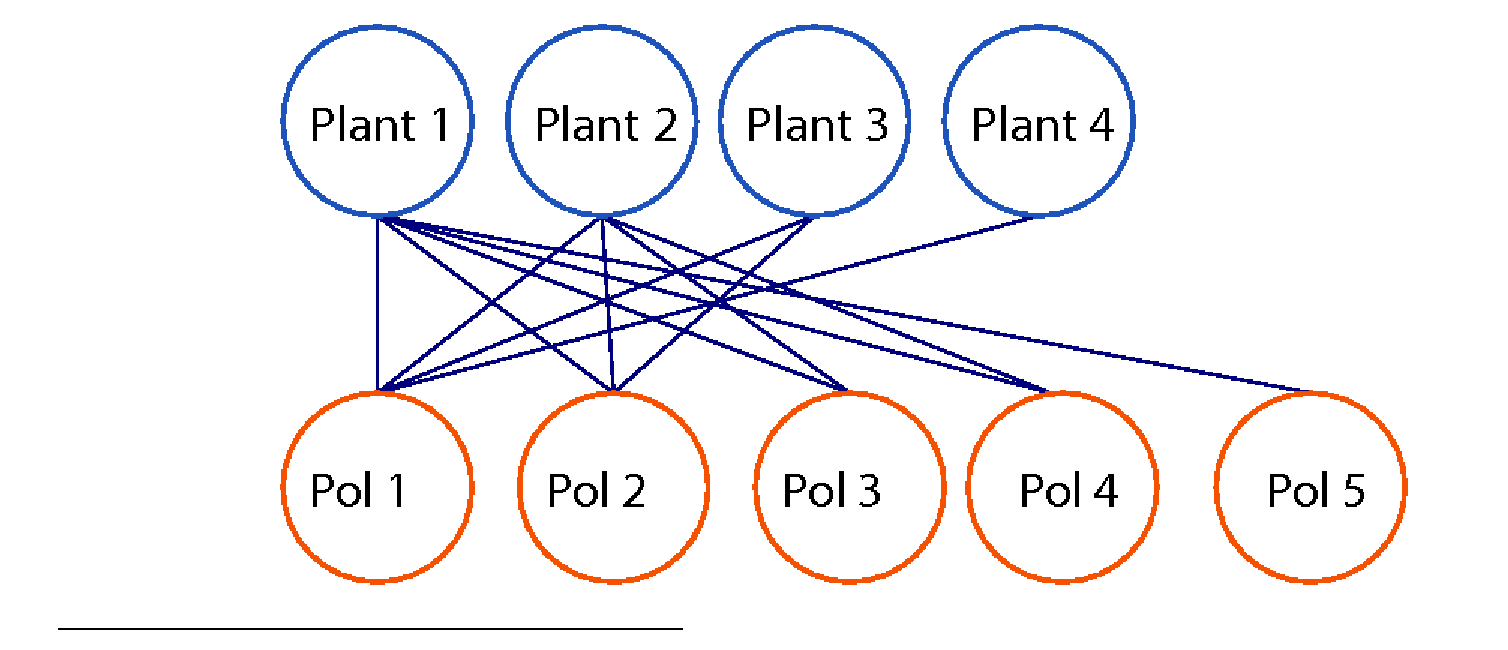
\includegraphics[scale=0.5]{DINAMICA_red_exper_stab2.eps}
\caption {Comunidad mutualista con cinco especie de plantas y cuatro de polinizadores.}
\label{fig:red_exper_stab1}
\end{figure}

La figura \ref{fig:red_exper_stab1} muestra una pequeña comunidad mutualista ficticia, que hemos construido para los experimentos numéricos. Este ejemplo sencillo muestra la dinámica característica de las redes reales.

\begin{figure}[ht!]
\centering
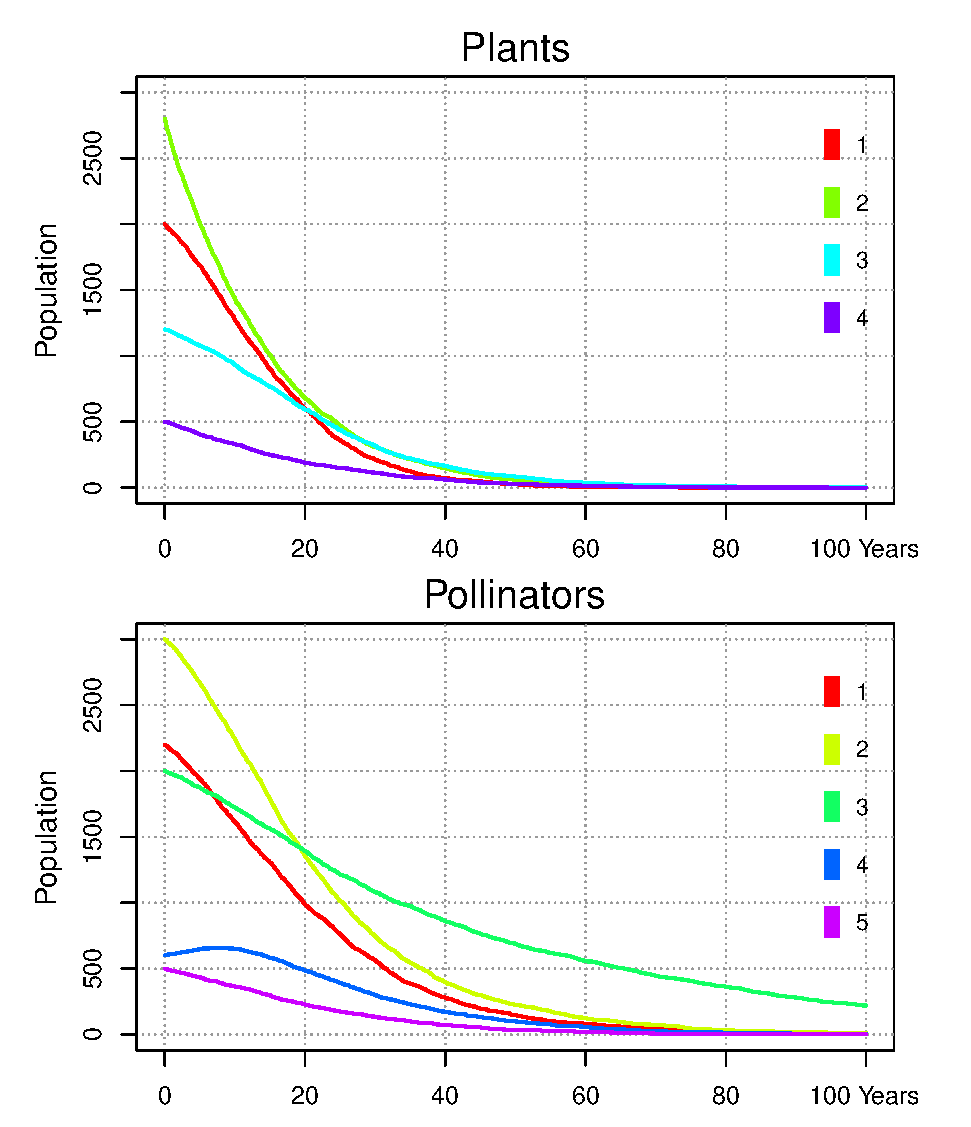
\includegraphics[width=8cm]{DINAMICA_Fig5_extinction.eps}
\caption {Dinámica de poblaciones para $4+5$ especies que termina en la extinción completa.}
\label{fig:exper_stab1}
\end{figure}

En el primer experimento el sistema empieza con todas las tasas efectivas negativas, excepto la del polinizador número $4$. Asumimos que el mutualismo es obligado. En estas circunstancias es sencillo encontrar los valores mínimos de población que garantizarían la supervivencia resolviendo $r_{\rm{eff}.i} = 0$ en las ecuaciones \eqref{modelors}, para todo $i$.

Las tasas efectivas solo pueden ser positivas por el beneficio mutualista, pero en esta simulación las poblaciones iniciales no son suficientes para para conseguirlo, con la excepción del mencionado polinizador número $4$. Las especies de planta $1$ y $2$ empiezan con poblaciones por encima de sus capacidades de carga.
Este experimento muestra el \textit{atractor de extinción} que conduce a la destrucción total de la comunidad.

\begin{figure}[ht!]
\centering
\includegraphics[scale = 0.66]{DINAMICA_Fig6_carrying_cap.eps}
\caption {Evolución temporal de las poblaciones y de las tasas de crecimiento efectivas del mismo sistema de $4+5$ species (figura \ref{fig:red_exper_stab1}). La comunidad termina con todas las especies en sus capacidades de carga respectivas.}
\label{fig:exper_carrying_cap}
\end{figure}

La figura \ref{fig:exper_carrying_cap} muestra un segundo experimento, con la misma red, pero con diferentes parámetros (Anexo \ref{DINAMICA_ANEXO_KConst}). En esta simulación, todas las poblaciones de plantas iniciales están por debajo de sus capacidades de carga, pero con tasas de crecimiento efectivas positivas, por lo que terminan en máximos. La población del polinizador $5$ está inicialmente por encima de su capacidad de carga, por eso la tasa efectiva es ligeramente negativa y converge hacia la capacidad de carga al final de la simulación. Por el contrario, la especie de polinizador $4$ tiene muy pocos individuos al principio pero la abundancia de mutualistas genera una tasa eficaz positiva y una curva tipo de crecimiento logístico. Al final de la simulación todas las tasas efectivas convergen a cero, es el atractor que aparece en el máximo de poblaciones.

\begin{figure}[h!]
\centering
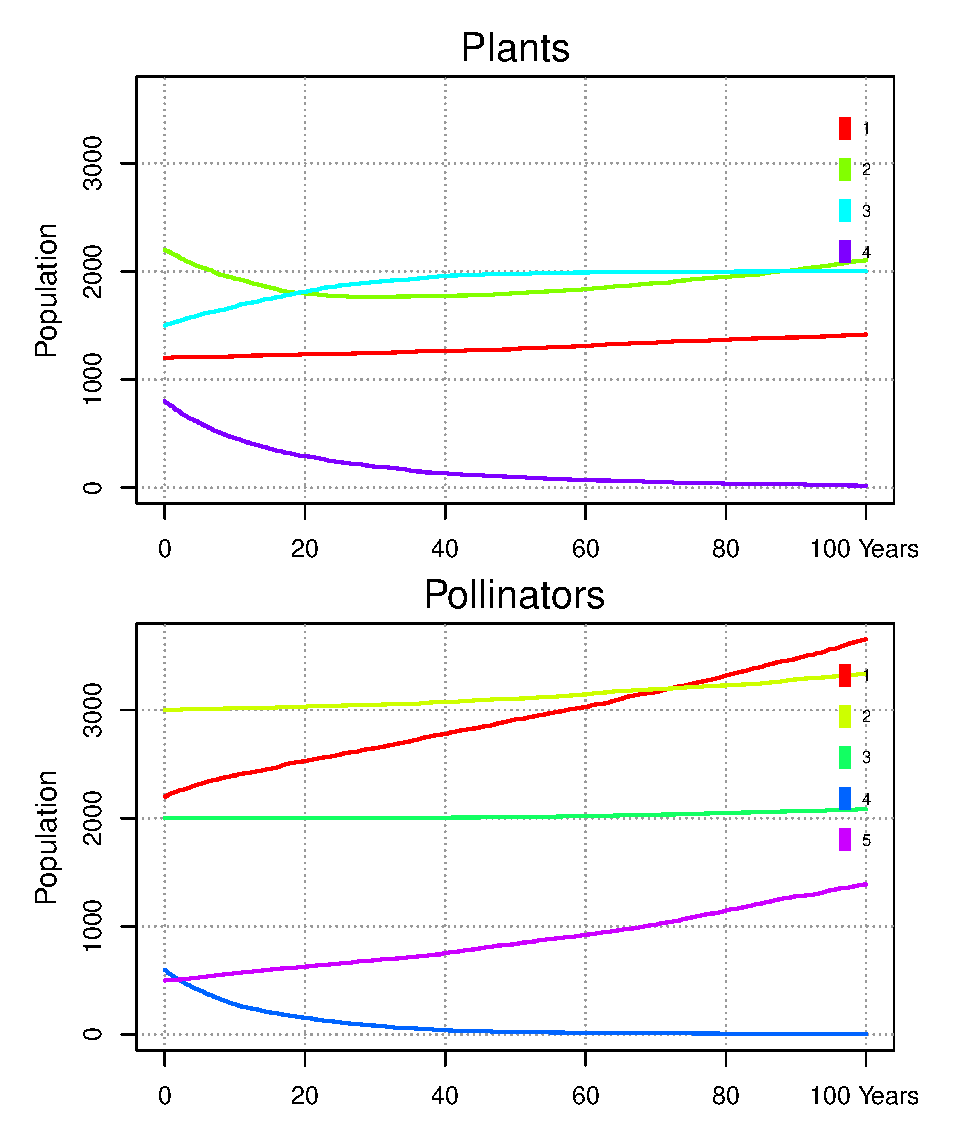
\includegraphics[scale = 0.66 ]{DINAMICA_Fig7_partial_extinct.eps}
\caption {Resultados del tercer experimento. El polinizador $4$ y la planta $4$ se extinguen.}
\label{fig:exper_stab2}
\end{figure}

En la tercera simulación exploramos las extinciones parciales (figure \ref{fig:exper_stab2}). De nuevo, todas las tasas vegetativas son negativas, pero los pesos de los enlaces se han modificado ligeramente respecto al experimento anterior.

En esta simulación todas las poblaciones empiezan por debajo de sus capacidades de carga. Todas evolucionan hacia sus máximos excepto el polinizador $4$ y la planta $4$ que se extinguen. La especie de planta $2$ empieza con una tasa eficaz negativa pero el crecimiento de sus mutualistas da la vuelta a esta situación y termina sobreviviendo.

\subsection{Simulaciones con saturación del beneficio}
\label{results_K_constante}

En este apartado presentamos los resultados de las simulaciones que hemos llevado a cabo con el modelo de saturación del beneficio mutualista (ecuaciones \ref{eq:DINAMICA_modeloralphaconmut}). Para el primer experimento hemos utilizado la misma red ficticia que en el apartado anterior (figura \ref{fig:red_exper_stab1})

\begin{figure}[b!]
\centering
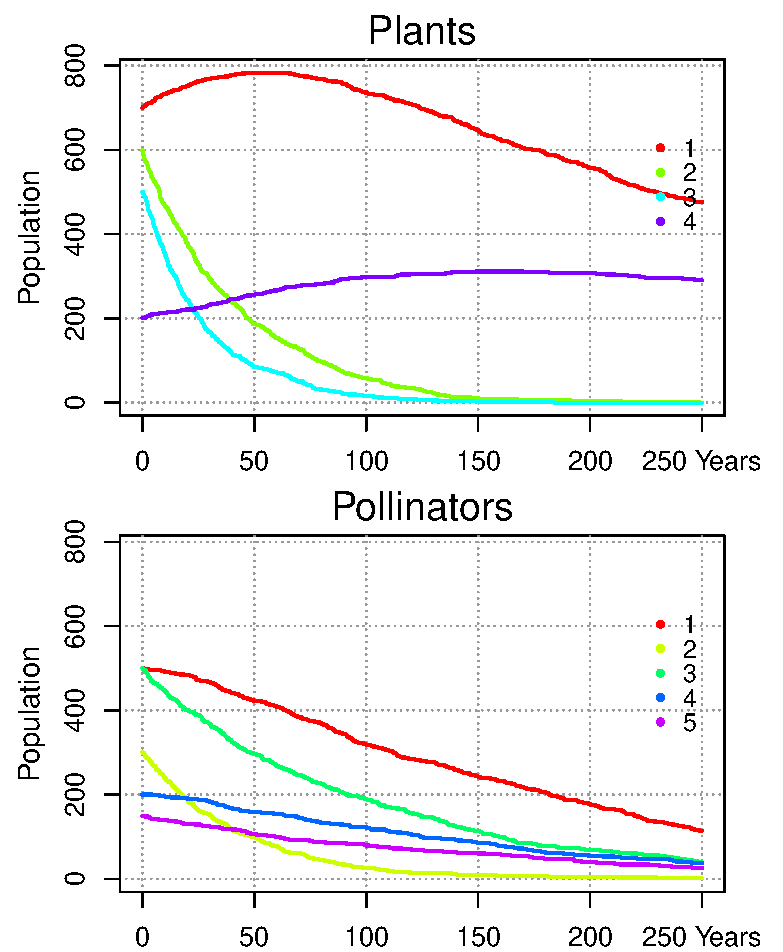
\includegraphics[scale=0.66]{DINAMICA_SATU_experimento_1.pdf}
\caption {Resultados del primer experimento. La parametrización puede verse en el Anexo \ref{DINAMICA_ANEXO_saturacion}, tabla \ref{tab:SAT_experiment1}.}
\label{fig:DINAMICA_SAT_exper_stab1}
\end{figure}

En todos los experimentos las tasas vegetativas son negativas, el mutualismo es obligado para todas las especies.

El primer experimento con saturación es similar al realizado para el modelo con capacidades de carga constantes. En este caso, hay especies que empiezan la simulación con tasas efectivas negativas y otras positivas, pero el sistema está al principio por debajo de la divisoria multidimensional y se extingue porque la trayectoria termina en el atractor de destrucción.

\begin{figure}[h!]
\centering
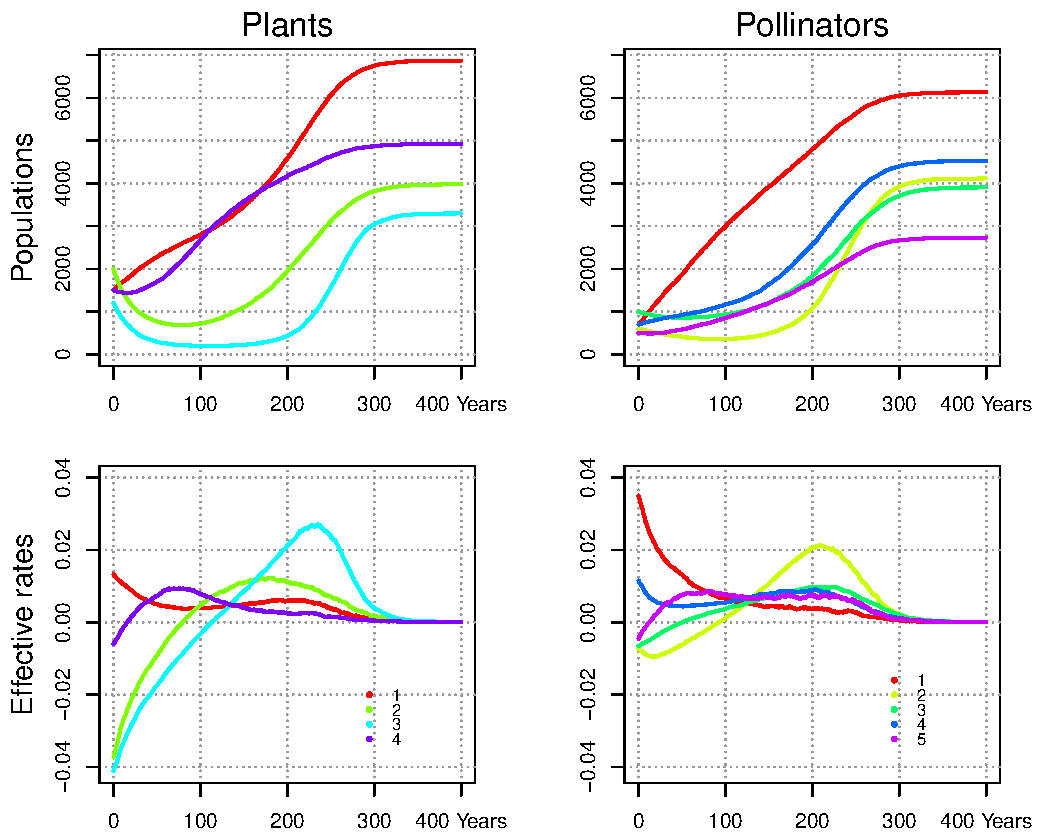
\includegraphics[scale=0.8]{DINAMICA_SATU_experimento_2.pdf}
\caption {Resultados del segundo experimento. La configuración puede consultarse en el Anexo  \ref{DINAMICA_ANEXO_saturacion}, tabla \ref{tab:SAT_experiment2}.}
\label{fig:DINAMICA_SAT_exper_stab2}
\end{figure}

La segunda simulación (figura \ref{fig:DINAMICA_SAT_exper_stab2}) muestra como el sistema evoluciona hasta máximos de todas las especies. En este caso resulta de gran interés ver como varían las tasas de crecimiento eficaces y la complejidad que pueden llegar a adquirir por las múltiples interacciones. Al final todas terminan anulándose porque el sistema ha alcanzado el punto de equilibrio máximo. 

Los análisis de estabilidad de este capítulo asumían que las condiciones no se alteran durante el estudio. En realidad, las tasas varían como consecuencia de diferentes perturbaciones medioambientales. A continuación, vamos a ver la resistencia del sistema ante perturbaciones externas, simulando fuerte incrementos en las tasas de mortalidad $r_{d_i}$ como las que producen las sequías o las enfermedades. La literatura afirma que el \emph{anidamiento} proporciona resistencia a las comunidades \citep{bascompte2003nested}. Los dos últimos experimentos muestran como influye esta magnitud.

\begin{figure}[h!]
\centering
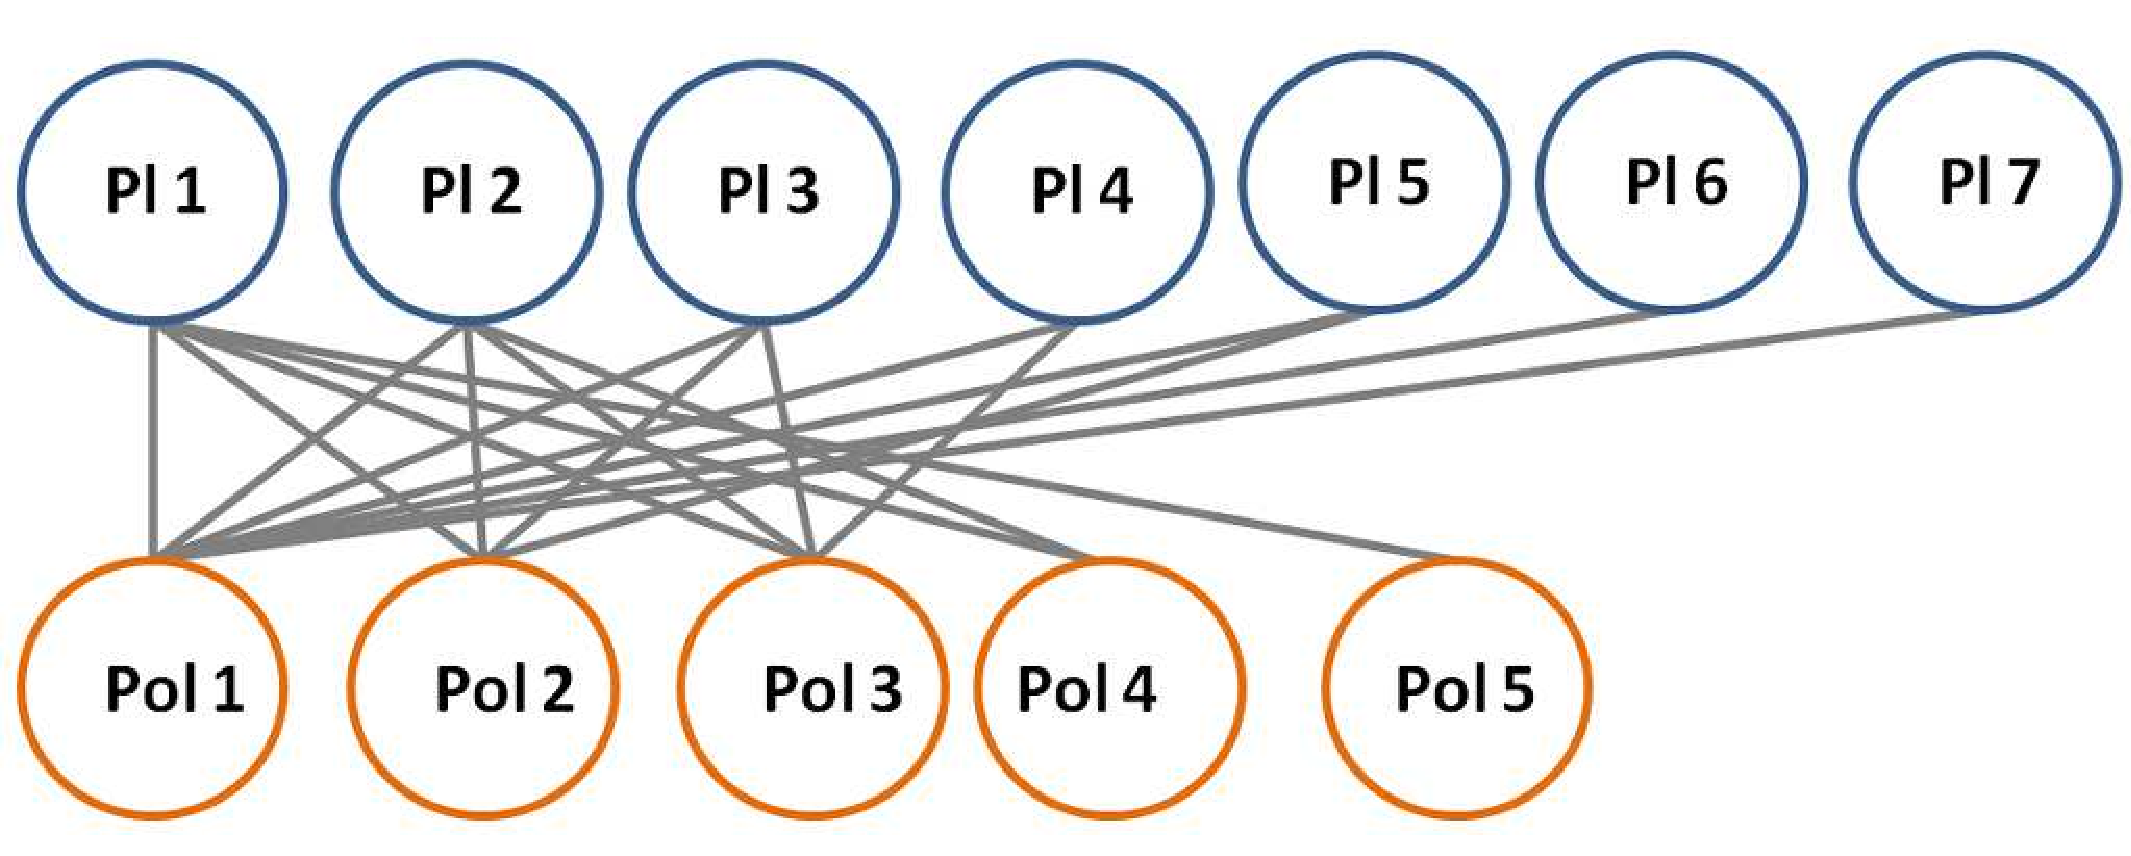
\includegraphics[scale=0.28]{DINAMICA_SAT_red_exper_resilience_strong.pdf}
\caption {Red con anidamiento fuerte. Tabla \ref{tab:SAT_exper_resilience_strong}.}
\label{fig:DINAMICA_SAT_red_exper_resilience_strong}
\end{figure}

En el penúltimo usamos otra red fictica, con siete especies de plantas y cinco de polinizadores (figura \ref{fig:DINAMICA_SAT_red_exper_resilience_strong}). Puede identificarse de manera visual el núcleo central de especies generalistas y las especies especialistas conectadas a generalistas de la clase contraria. Se han elegido las poblaciones iniciales para que el sistema esté en la cuenca de supervivencia.

\begin{figure}[h!]
\centering
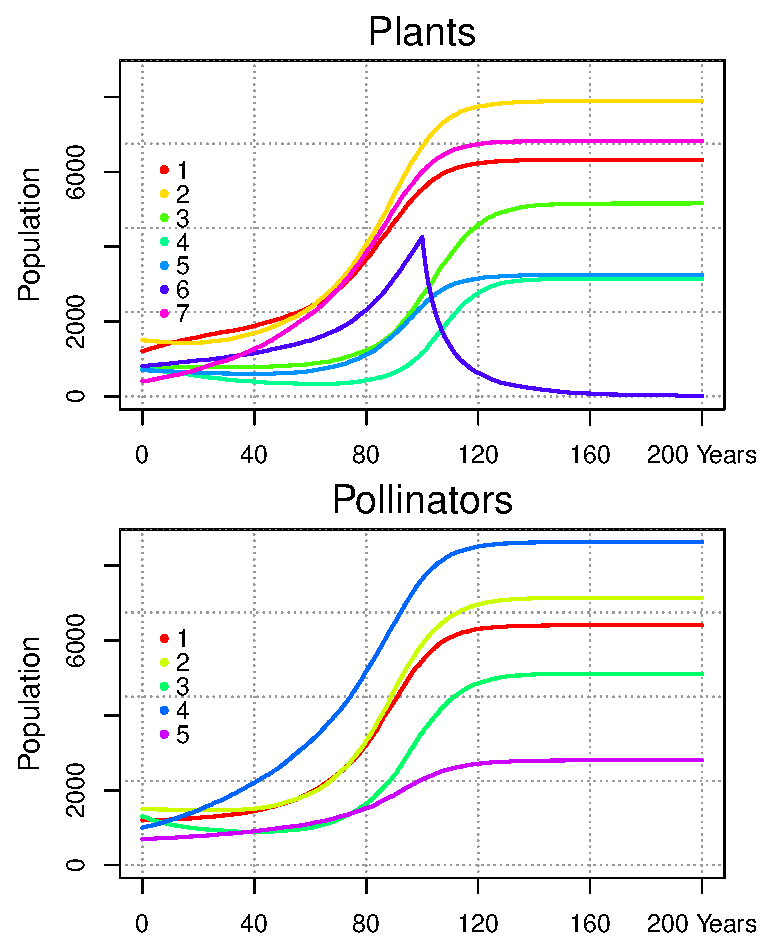
\includegraphics[scale=0.75]{DINAMICA_SATU_nested.pdf}
\caption {Experimento con la red con anidamiento fuerte. Una perturbación externa ataca la especie de planta número $6$. Tabla \ref{tab:SAT_exper_resilience_strong}.}
\label{fig:DINAMICA_SAT_exper_resilience_strong}
\end{figure}

El sistema crecería hasta alcanzar máximos en ausencia de perturbaciones externas, pero la especie $6$ de plantas sufre un aumento abrupto de mortalidad de un $20\%$ anual que la conduce a la extinción. Esta especie estaba conectada solo al polinizador $1$, el más generalista de su clase. El efecto de la extinción es despreciable sobre este polinizador porque el resto de especies benefactoras lo suplen. 

\begin{figure}[h!]
\centering
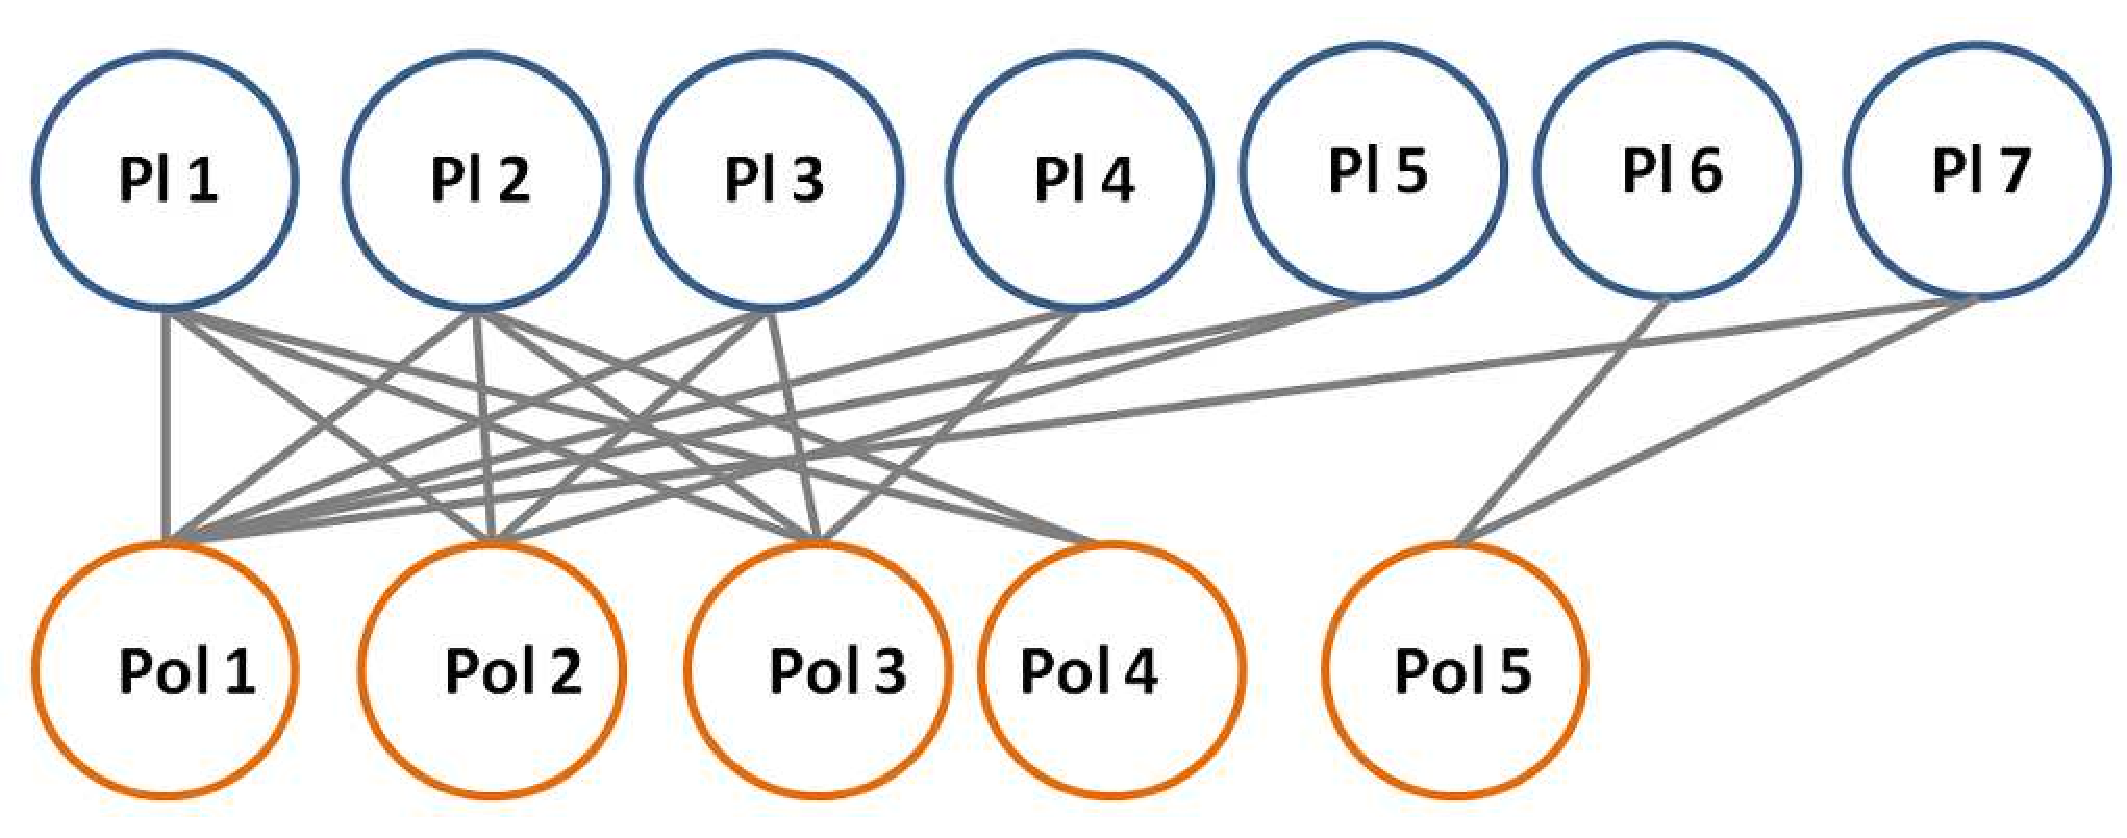
\includegraphics[scale=0.28]{DINAMICA_SAT_red_exper_resilience_weak.pdf}
\caption {Red débilmente anidada. Tabla \ref{tab:SAT_exper_resilience_weak}.}
\label{fig:DINAMICA_SAT_red_exper_resilience_weak}
\end{figure}

El último experimento usa una red ligeramente modificada (figura\ref{fig:DINAMICA_SAT_red_exper_resilience_weak}). La especie de plantas $6$ se conecta al polinizador $5$, un especialista. También se elimina el enlace que conecta la planta $1$ con el polinizador $5$ y se reemplaza por uno nuevo entre la planta $7$ y el polinizador $1$.  

\begin{figure}[h!]
\centering
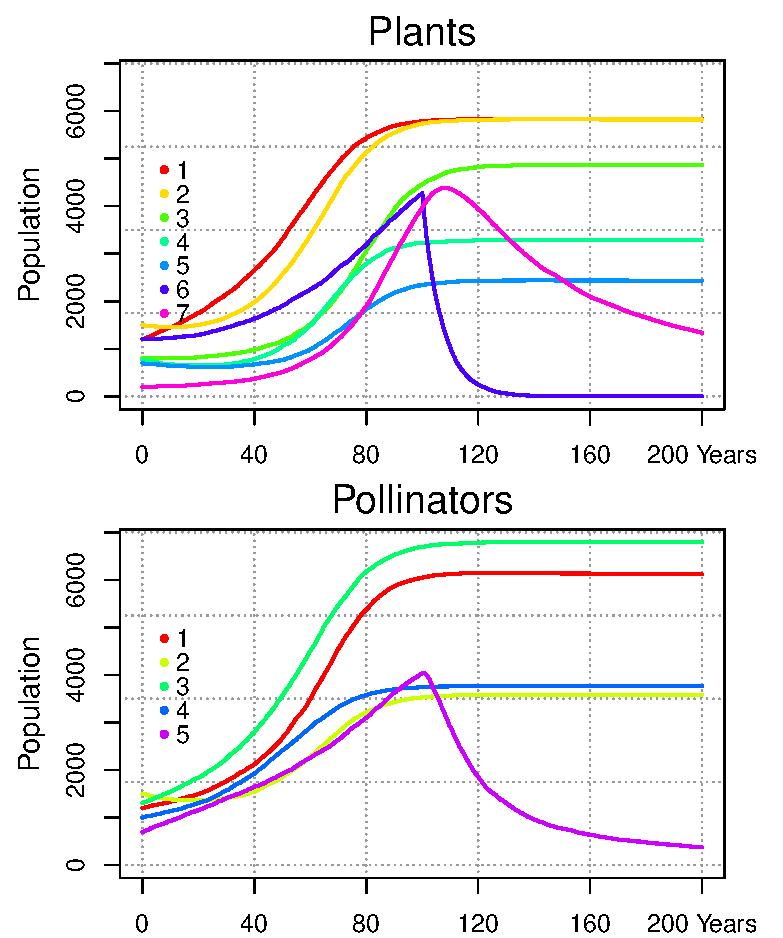
\includegraphics[scale=0.75]{DINAMICA_SATU_weak.pdf}
\caption {Experimento con una red menos anidada. Una perturbación externa ataca la planta $6$. Tabla \ref{tab:SAT_exper_resilience_weak}.}
\label{fig:DINAMICA_SAT_exper_resilience_weak}
\end{figure}

Las posibilidades de supervivencia de una nueva especie que llegue a la comunidad son mayores si se conecta con una generalista. Este propiedad se debe no solo al hecho de que las generalistas son menos vulnerables por la gran cantidad de especies de las que reciben beneficio. Enlazarse con una especialista expone a la destrucción por arrastre.

Cuando la planta $6$ es atacada y se extingue el efecto es mucho peor para la red. El polinizador $5$ pierde a su única especie benefactora, de manera que su tasa efectiva se vuelve negativa y finalmente desaparecerá. La planta $7$, conectada con el polinizador $5$ también se ve condenada a la extinción porque su enlace con el polinizador $1$ no compensa la pérdida. En resumen, una perturbación externa sobre la especie de planta $6$ arrastra a la extinción a la planta $7$ por culpa del enlace que comparten con el polinizador $5$. Si ambas plantas compartieran enlaces con el núcleo generalista esta destrucción en cascada resultaría mucho más improbable.

\section{Conclusiones}

Nunc posuere quam at lectus tristique eu ultrices augue venenatis. Vestibulum ante ipsum primis in faucibus orci luctus et ultrices posuere cubilia Curae; Aliquam erat volutpat. Vivamus sodales tortor eget quam adipiscing in vulputate ante ullamcorper. Sed eros ante, lacinia et sollicitudin et, aliquam sit amet augue. In hac habitasse platea dictumst.

\clearpage
\section{Anexo: Datos de las simulaciones del modelo con \textit{K} constantes}
\label{DINAMICA_ANEXO_KConst}

\begin{table}[h!]
\centering
\footnotesize
\begin{tabular}{lrrrr}
\hline
 & Planta 1 & Planta 2 & Planta 3 & Planta 4  \\
\hline
\\
$b_{pol1j}\left(10^{-6}\right)$ & 1 & 12 & 12 & 16 \\
$b_{pol2j}\left(10^{-6}\right)$ & 20 & 4 & 11 & 0 \\
$b_{pol3j}\left(10^{-6}\right)$ & 20 & 10 & 0 & 0 \\
$b_{pol4j}\left(10^{-6}\right)$ & 10 & $0.1$ & 0 & 0 \\
$b_{pol5j}\left(10^{-6}\right)$ & 10 & 0 & 0 & 0 \\
$N_{init\,j}$ & 2000 & 2800 & 1200 & 500 \\
$K_{j}$ & 1500 & 2500 & 2000 & 1000 \\
$r_{birth\, j}$ & 0.004 & 0.01 & 0.01 & 0.005 \\
$r_{death\, j}$ & 0.13 & 0.10 & 0.08 & 0.065 \\
\hline
\\
\end{tabular}

\begin{tabular}{lrrrrr}
\hline
 &Pol 1&Pol 2&Pol 3&Pol 4&Pol 5\\
\hline
\\
$b_{pl1m}\left(10^{-6}\right)$ & 4 & 13 & 5 & 30 & 20\\
$b_{pl2m}\left(10^{-6}\right)$ & 12 & 6 & 10 & $0.1$ & 0\\
$b_{pl3m}\left(10^{-6}\right)$ & 2 & 5 & 0 & 0 & 0\\
$b_{pl4m}\left(10^{-6}\right)$ & 10 & 0 & 0 & 0 & 0\\
$N_{init\,m}$ & 3000 & 3000 & 2000 & 600 & 500 \\
$K_{m}$& 5000 & 4000 & 3000 & 2000 & 2000\\
$r_{b\, m}$ & 0.08 & 0.02 & 0.05 & 0.08 & 0.02 \\
$r_{d\, m}$ & 0.14 & 0.078 & 0.07 & 0.14 & 0.08 \\
\hline
\end{tabular}
\normalsize
\caption{Coeficientes mutualistas y condiciones del primer experimento del modelo con capacidades de carga constantes (fig. \ref{fig:exper_stab1}), con la red de la figura \ref{fig:red_exper_stab1}. Arriba, la matriz polinizador-planta, abajo la planta-polinizador.}
\label{tab:experiment1}\vspace*{-10pt}
\end{table}

\begin{table}[h!]
\centering
\footnotesize
\begin{tabular}{lrrrr}
\hline
 & Planta 1 & Planta 2 & Planta 3 & Planta 4  \\
\hline
\\
$b_{pol1j}\left(10^{-6}\right)$ & 50 & 22 & 42 & 56 \\
$b_{pol2j}\left(10^{-6}\right)$ & 20 & 40 & 81 & 0 \\
$b_{pol3j}\left(10^{-6}\right)$ & 20 & 10 & 0 & 0 \\
$b_{pol4j}\left(10^{-6}\right)$ & 50 & $0.1$ & 0 & 0 \\
$b_{pol5j}\left(10^{-6}\right)$ & 10 & 0 & 0 & 0 \\
$N_{init\,j}$ & 1500 & 1200 & 1000 & 500 \\
$K_{j}$ & 2800 & 2500 & 2000 & 1000 \\

\hline
\\
\end{tabular}

\begin{tabular}{lrrrrr}
\hline
 &Pol 1&Pol 2&Pol 3&Pol 4&Pol 5\\
\hline
\\
$b_{pl1m}\left(10^{-6}\right)$ & 40 & 13 & 15 & 30 & 20\\
$b_{pl2m}\left(10^{-6}\right)$ & 12 & 6 & 1 & 1 & 0\\
$b_{pl3m}\left(10^{-6}\right)$ & 2 & 5 & $0.1$ & 0 & 0\\
$b_{pl4m}\left(10^{-6}\right)$ & 1 & 1 & 0 & 0 & 0\\
$N_{init\,m}$ & 2200 & 3000 & 2000 & 600 & 2200 \\
$K_{m}$& 5000 & 4000 & 3000 & 2000 & 2000\\
\hline
\end{tabular}
\normalsize
\caption{Configuración del experimento de la figura \ref{fig:exper_stab2} Las tasas de nacimiento y muerte son las mismas que en la tabla \ref{tab:experiment1} excepto $r_{d,pl3}=0.1$, $r_{d,pol2}=0.048$ y $r_{d,pol5}=0.04$}
\label{tab:experiment2}
\end{table}


\begin{table}[h!]
\centering
\footnotesize
\begin{tabular}{lrrrr}
\hline
 & Planta 1 & Planta 2 & Planta 3 & Planta 4  \\
\hline
\\
$b_{pol1j}\left(10^{-6}\right)$ & 10 & 22 & 42 & 6 \\
$b_{pol2j}\left(10^{-6}\right)$ & 20 & 4 & 11 & 0 \\
$b_{pol3j}\left(10^{-6}\right)$ & 20 & 10 & 0 & 0 \\
$b_{pol4j}\left(10^{-6}\right)$ & 1 & $0.1 $ & 0 & 0 \\
$b_{pol5j}\left(10^{-6}\right)$ & 1 & 0 & 0 & 0 \\
$N_{init\,j}$ & 1200 & 2200 & 1500 & 800 \\
$K_{j}$ & 1500 & 2500 & 2000 & 1000 \\

\hline
\\
\end{tabular}

\begin{tabular}{lrrrrr}
\hline
 &Pol 1&Pol 2&Pol 3&Pol 4&Pol 5\\
\hline
\\
$b_{pl1m}\left(10^{-6}\right)$ & 34 & 33 & 15 & 20 & 60\\
$b_{pl2m}\left(10^{-6}\right)$ & 12 & 6 & 1 & $0.1$ & 0\\
$b_{pl3m}\left(10^{-6}\right)$ & 2 & 5 & 0 & 0 & 0\\
$b_{pl4m}\left(10^{-6}\right)$ & 1 & $0.1$ & 0 & 0 & 0\\
$N_{init\,m}$ & 2200 & 3000 & 2000 & 600 & 2200 \\
$K_{m}$& 5000 & 4000 & 3000 & 2000 & 2000\\
\hline
\end{tabular}
\normalsize
\caption{Configuración del tercer experimento numérico (figura \ref{fig:exper_stab2})  Las tasas de nacimiento y muerte son las mismas que en la tabla \ref{tab:experiment1} excepto  $r_{d,pl4}=0.053$, $r_{d,pol4}=0.09$ y $r_{b,pol4}=0.01$}
\label{tab:experiment3}
\end{table}

\section{Anexo: Datos de las simulaciones del modelo con saturación}
\label{DINAMICA_ANEXO_saturacion}

\begin{table}[h!]
\centering
\footnotesize
\begin{tabular}{lrrrr}
\hline
 & Planta 1 & Planta 2 & Planta 3 & Planta 4  \\
\hline
$b_{1j}${\tiny $\left(10^{-6}\right)$} & 1 & 12 & 12 & 16\\
$b_{2j}${\tiny $\left(10^{-6}\right)$} & 12 & 4 & 11 & 0 \\
$b_{3j}${\tiny $\left(10^{-6}\right)$} & 12 & 10 & 0 & 0 \\
$b_{4j}${\tiny $\left(10^{-6}\right)$} & 6 & 10 & 0 & 0 \\
$b_{5j}${\tiny $\left(10^{-6}\right)$} & 10 & 0 & 0 & 0 \\
$N_{init\,j}$ & 700 & 600 & 500 & 200 \\
$c_{j}${\tiny $\left(10^{-4}\right)$} & 1 & 1 & 1 & 1 \\
$\alpha_{j}${\tiny $\left(10^{-6}\right)$} & 7 & 12 & 12 & 10 \\
$r_{birth\, j}$ & 0.004 & 0.01 & 0.01 & 0.005 \\
$r_{death\, j}$ & 0.005 & 0.04 & 0.05 & 0.0055 \\
\hline
\\
\end{tabular}
\begin{tabular}{lrrrrr}
\hline
 &Pol 1&Pol 2&Pol 3&Pol 4&Pol 5\\
\hline
$b_{1m}${\tiny $\left(10^{-6}\right)$}&14&13&10&10&20\\
$b_{2m}${\tiny $\left(10^{-6}\right)$}&12&6&1&10&0\\
$b_{3m}${\tiny $\left(10^{-6}\right)$}&2&5&1&0&0\\
$b_{4m}${\tiny $\left(10^{-6}\right)$}&10&1&0&0&0\\
$N_{init\,m}$ & 500 & 300 & 500 & 200 & 150 \\
$c_{m}${\tiny $\left(10^{-4}\right)$} & 1 & 1 & 1 & 1 & 1\\
$\alpha_{m}${\tiny $\left(10^{-6}\right)$} & 10 & 10 & 8 & 10 & 30\\
$r_{b\, m}$ & 0.28 & 0.02 & 0.05 & 0.02 & 0.02 \\
$r_{d\, m}$ & 0.44 & 0.058 & 0.065 & 0.034 & 0.038 \\
\hline
\end{tabular}
\normalsize
\caption{Coeficientes y condiciones del primer experimento con saturación del beneficio (figura \ref{fig:DINAMICA_SAT_exper_stab1}), con la red de la figura \ref{fig:red_exper_stab1}. Arriba, la matriz polinizador-planta; abajo la matriz planta-polinizador.}

\label{tab:SAT_experiment1}
\end{table}
\begin{table}[hp]
\centering
\footnotesize
\begin{tabular}{lrrrr}
\hline
 & Planta 1 & Planta 2 & Planta 3 & Planta 4  \\
\hline
$b_{1j}${\tiny $\left(10^{-6}\right)$} & 1 & 12 & 12 & 16\\
$b_{2j}${\tiny $\left(10^{-6}\right)$} & 12 & 4 & 11 & 0 \\
$b_{3j}${\tiny $\left(10^{-6}\right)$} & 12 & 10 & 0 & 0 \\
$b_{4j}${\tiny $\left(10^{-6}\right)$} & 6 & 10 & 0 & 0 \\
$b_{5j}${\tiny $\left(10^{-6}\right)$} & 10 & 0 & 0 & 0 \\
$N_{init\,j}$ & 1500 & 2000 & 1200 & 1500 \\
$c_{j}${\tiny $\left(10^{-4}\right)$} & 1 & 1 & 1 & 1 \\
$\alpha_{j}${\tiny $\left(10^{-6}\right)$} & 7 & 12 & 12 & 10 \\
$r_{birth\, j}$ & 0.004 & 0.01 & 0.01 & 0.005 \\
$r_{death\, j}$ & 0.005 & 0.04 & 0.05 & 0.0055 \\
\hline
\\
\end{tabular}
\centering
\begin{tabular}{lrrrrr}
\hline
 &Pol 1&Pol 2&Pol 3&Pol 4&Pol 5\\
\hline
$b_{1m}${\tiny $\left(10^{-6}\right)$}&14&13&10&10&20\\
$b_{2m}${\tiny $\left(10^{-6}\right)$}&12&6&1&10&0\\
$b_{3m}${\tiny $\left(10^{-6}\right)$}&2&5&1&0&0\\
$b_{4m}${\tiny $\left(10^{-6}\right)$}&10&1&0&0&0\\
$N_{init\,m}$ & 700 & 600 & 1000 & 700 & 500 \\
$c_{m}${\tiny $\left(10^{-4}\right)$} & 1 & 1 & 1 & 1 & 1\\
$\alpha_{m}${\tiny $\left(10^{-6}\right)$} & 10 & 10 & 8 & 10 & 30\\
$r_{b\, m}$ & 0.28 & 0.02 & 0.05 & 0.02 & 0.02 \\
$r_{d\, m}$ & 0.44 & 0.058 & 0.065 & 0.034 & 0.038 \\
\hline
\end{tabular}
\normalsize
\caption{Coeficientes y condiciones del segundo experimento con saturación del beneficio (figura \ref{fig:DINAMICA_SAT_exper_stab2}). Arriba, la matriz polinizador-planta; abajo la matriz planta-polinizador.}
\label{tab:SAT_experiment2}
\end{table}

\begin{table}
\centering
\scriptsize
\begin{tabular}{lrrrrrrr}
\hline
 &Planta 1&Planta 2&Planta 3&Planta 4&Planta 5&Planta 6&Planta 7\\
\hline
$b_{1j\, }${\tiny $\left(10^{-6}\right)$}&20&12&16&16&19&25&35\\
$b_{2j\, }${\tiny $\left(10^{-6}\right)$}&12&14&4.1&2&22&0&0\\
$b_{3j\, }${\tiny $\left(10^{-6}\right)$}&20&11&3.1&20&0&0&0\\
$b_{4j\, }${\tiny $\left(10^{-6}\right)$}&11&24&0&0&0&0&0\\
$b_{5j\, }${\tiny $\left(10^{-6}\right)$}&1&0&0&0&0&0&0\\
$N_{init\,j}$&1200 & 1500 & 800 & 770 & 700 & 800 & 400\\
$c_{j}${\tiny $\left(10^{-4}\right)$} & 1 & 0.5 & 1 & 2 & 1 & 1 & 1\\
$\alpha_{j}${\tiny $\left(10^{-6}\right)$} & 20 & 30 & 10 & 10 & 50 & 10 &10\\
$r_{birth\, j}$ & 0.004 & 0.01 & 0.02 & 0.005 & 0.004 & 0.02 & 0.025\\
$r_{death\, j}$ & 0.03 & 0.04 & 0.04 & 0.055 & 0.03 & 0.03 & 0.028\\
\hline
\\
\end{tabular}
\centering
\begin{tabular}{lrrrrr}
\hline
 &Pol 1&Pol 2&Pol 3&Pol 4&Pol 5\\
\hline
$b_{1m\,}${\tiny $\left(10^{-6}\right)$}&14&13&23&30&23\\
$b_{2m\,}${\tiny $\left(10^{-6}\right)$}&19&26&10&10&0\\
$b_{3m\,}${\tiny $\left(10^{-6}\right)$}&2&25&10&0&0\\
$b_{4m\,}${\tiny $\left(10^{-6}\right)$}&1&11&10&0&0\\
$b_{5m\,}${\tiny $\left(10^{-6}\right)$}&1&1&0&0&0\\
$b_{6m}${\tiny $\left(10^{-6}\right)$}&1&0&0&0&0\\
$b_{7m}${\tiny $\left(10^{-6}\right)$}&1&0&0&0&0\\
$N_{init\,m}$ & 1200 & 1500 & 1300 & 1000 & 700 \\
$c_{m}${\tiny $\left(10^{-4}\right)$} & 1 & 1 & 1 & 0.7 & 2\\
$\alpha_{m}${\tiny $\left(10^{-6}\right)$} & 10 & 10 & 20 & 10 & 20\\
$r_{b\, m}$ & 0.08 & 0.02 & 0.02 & 0.05 & 0.02 \\
$r_{d\, m}$ & 0.11 & 0.078 & 0.068 & 0.07 & 0.028 \\
\hline
\end{tabular}
\normalsize
\caption{Coeficientes y condiciones para el experimento con la red fuertemente anidada (figura \ref{fig:DINAMICA_SAT_red_exper_resilience_strong}). Arriba, la matriz polinizador-planta; abajo la matriz planta-polinizador.}
\label{tab:SAT_exper_resilience_strong}
\end{table}

\begin{table}[h!]
\centering
\scriptsize
\begin{tabular}{lrrrrrrr}
\hline
 &Planta 1&Planta 2&Planta 3&Planta 4&Planta 5&Planta 6&Planta 7\\
\hline
$b_{1j\, }${\tiny $\left(10^{-6}\right)$}&20&12&16&16&19&0&45\\
$b_{2j\, }${\tiny $\left(10^{-6}\right)$}&12&14&4.1&2&22&0&0\\
$b_{3j\, }${\tiny $\left(10^{-6}\right)$}&20&11&3.1&20&0&0&0\\
$b_{4j\, }${\tiny $\left(10^{-6}\right)$}&11&24&0&0&0&0&0\\
$b_{5j\, }${\tiny $\left(10^{-6}\right)$}&0&0&0&0&0&25&1\\
$N_{init\,j}$&1200 & 1500 & 800 & 770 & 700 & 400 &1000\\
$c_{j}${\tiny $\left(10^{-4}\right)$} & 1 & 0.5 & 1 & 2 & 1 & 1 & 1\\
$\alpha_{j}${\tiny $\left(10^{-6}\right)$} & 20 & 30 & 10 & 10 & 50 & 10 &10\\
$r_{birth\, j}$ & 0.004 & 0.01 & 0.02 & 0.005 & 0.004 & 0.02 & 0.025\\
$r_{death\, j}$ & 0.03 & 0.04 & 0.04 & 0.055 & 0.03 & 0.024 & 0.04\\
\hline
\\
\end{tabular}
\begin{tabular}{lrrrrr}
\hline
 &Pol 1&Pol 2&Pol 3&Pol 4&Pol 5\\
\hline
$b_{1m\,}${\tiny $\left(10^{-6}\right)$}&14&13&23&30&0\\
$b_{2m\,}${\tiny $\left(10^{-6}\right)$}&19&26&10&10&0\\
$b_{3m\,}${\tiny $\left(10^{-6}\right)$}&2&25&10&0&0\\
$b_{4m\,}${\tiny $\left(10^{-6}\right)$}&1&11&10&0&0\\
$b_{5m\,}${\tiny $\left(10^{-6}\right)$}&1&1&0&0&0\\
$b_{6m}${\tiny $\left(10^{-6}\right)$}&0&0&0&0&5\\
$b_{7m}${\tiny $\left(10^{-6}\right)$}&1&0&0&0&30\\
$N_{init\,m}$ & 1200 & 1500 & 1300 & 1000 & 700 \\
$c_{m}${\tiny $\left(10^{-4}\right)$} & 1 & 1 & 1 & 0.7 & 2\\
$\alpha_{m}${\tiny $\left(10^{-6}\right)$} & 10 & 10 & 20 & 10 & 20\\
$r_{b\, m}$ & 0.09 & 0.02 & 0.02 & 0.05 & 0.02 \\
$r_{d\, m}$ & 0.11 & 0.058 & 0.04 & 0.07 & 0.025 \\
\hline
\end{tabular}
\normalsize
\caption{Coeficientes y condiciones para el experimento con la red débilmente anidada (figura \ref{fig:DINAMICA_SAT_red_exper_resilience_weak}). Arriba, la matriz polinizador-planta; abajo la matriz planta-polinizador.}
\label{tab:SAT_exper_resilience_weak}
\end{table}



\section{Anexo: Análisis de la estabilidad en detalle}
\label{DINAMICA_ANEXO_estabilidad}

Para simplificar, prescindimos de los superíndices que representan las clases $animal$ y $planta$. 
El sistema de ecuaciones \ref{eq:DINAMICA_dos_especies} se desarrolla en serie de Taylor en la vecindad del punto singular ($N^{*}_{1}, N^{*}_{2}$) como  $N_{1}= N^{*}_1+\tilde{N}_{1}$ y $N_{2}= N^{*}_2+\tilde{N}_{2}$ \cite{murray1993mathematical}:

\begin{equation}
\begin{array}{lcr}
\displaystyle \frac{d\tilde{N}_{1}}{dt} = r_{1}+ b_{12}(N^{*}_2+\tilde{N}_{2})-(\alpha_{1}+ c_{1} b_{12} (N^{*}_2+\tilde{N}_{2}))( N^{*}_1+\tilde{N}_{1})\nonumber\\
\\
\displaystyle \frac{d\tilde{N}_{2}}{dt} = r_{2}+ b_{21}( N^{*}_1+\tilde{N}_{1})-(\alpha_{2}+ c_{2} b_{21}(N^{*}_1+\tilde{N}_{1}))(N^{*}_2+\tilde{N}_{2}) 
\stepcounter{equation}\tag{\theequation}\label{eq:effrateTaylor}
\end{array}
\end{equation}

\noindent y quedándonos solo con los términos de primer orden:

\begin{equation}
\begin{array}{lcr}
\displaystyle \frac{d\tilde{N}_{1}}{dt}= \tilde{N}_{2}( b_{12} - c_{1} b_{12}\, N^{*}_1)-\tilde{N}_{1}(\alpha_{1}+ c_{1} b_{12} \, N^{*}_2) \equiv f_{1}(\tilde{N}_{1},\tilde{N}_{2}) \nonumber\\
\\
\displaystyle \frac{d\tilde{N}_{2}}{dt} = \tilde{N}_{1}( b_{21} - c_{2} b_{21}\, N^{*}_2)-\tilde{N}_{2}(\alpha_{2}+ c_{2} b_{21} \, N^{*}_1) \equiv f_{2}(\tilde{N}_{1},\tilde{N}_{2})
\stepcounter{equation}\tag{\theequation}\label{eq:effrateTaylor2}
\end{array}
\end{equation}

\noindent Los términos del jacobiano son:

\begin{equation}
\begin{array}{l}
J_{11}= \frac{\partial f_{1}}{\partial \tilde{N}_{1}} =- N^{*}_{1}\left(\alpha_{1}+ c_{1} b_{12} \, N^{*}_2\right)  \\
\\
J_{12}= \frac{\partial f_{1}}{\partial \tilde{N}_{2}} = N^{*}_{1}b_{12}\left(1 - c_{1}\, N^{*}_1\right) \\
\\
J_{21}= \frac{\partial f_{2}}{\partial \tilde{N}_{1}} = N^{*}_{2}b_{21} \left(1 - c_{2}\, N^{*}_2\right) \\
\\
J_{22}= \frac{\partial f_{2}}{\partial \tilde{N}_{2}} = - N^{*}_{2}\left(\alpha_{2}+ c_{2} b_{21}\,N^{*}_{1}\right)
\end{array}
\stepcounter{equation}\tag{\theequation}\label{eq:J11}
\end{equation}

\noindent que puede reescribirse en términos de los coeficientes positivos $J_{ij}$ como:

\begin{equation*}
J = \left(
\begin{array}{rr}
-J_{11} & J_{12} \\ J_{21} & -J_{22}
\end{array}
\right)
\end{equation*}

\noindent Los autovalores $\lambda_{1,2}$ se obtienen de
\begin{equation}
\lvert J - \lambda I \rvert =0
\stepcounter{equation}\tag{\theequation}\label{eq:lambda0App}
\end{equation}

\noindent cuyas soluciones son
\begin{equation}
\begin{array}{lcl}
\lambda _{1,2}=\frac{1}{2}\left(tr(J)\pm \sqrt{tr^{2}(J)-4\,\mathrm{Det}(J)}\right)\\ =
\frac{1}{2}\left(-\left(J_{11}+J_{22}\right)\pm \sqrt{\left(J_{11}+J_{22}\right)^{2}-4\,\mathrm{Det}(J)}\right)\\  =
\frac{1}{2}\left(-\left(J_{11}+J_{22}\right)\pm \sqrt{\left(J_{11}-J_{22}\right)^{2} +4 \,\left( J_{12}J_{21} \right) }\right)
\end{array}
\stepcounter{equation}\tag{\theequation}\label{eq:lambda12}
\end{equation}

\noindent La última expresión indica que los dos autovalores son reales. Además, satisfacen la siguiente condición:

\begin{equation}
\prod_{k}\lambda_{k}=\mathrm{Det}(J)
\end{equation}

\noindent por tanto el punto singular será un \textit{saddle} cuando se cumpla que  $\mathrm{Det}(J)<0$. Expandiendo el determinante del jacobiano obtenemos la condición de existencia del \textit{saddle}:

\begin{equation}
1-c_{1}N^{*}_{1}-c_{2}N^{*}_{2} >0
\end{equation}

Las extinciones parciales son también puntos singulares, y corresponden a $N^{*}_{1,2} = 0$. Para simplificar, escribimos solo las ecuaciones del punto singular  ($N^{*}_{1}=r_{1}/\alpha_{1},N^{*}_{2}=0$). Expandiendo en serie de Taylor en torno a él, el sistema de ecuaciones se convierte en:

\begin{equation}
\begin{array}{ll}
\displaystyle \frac{d\tilde{N}_{1}}{dt} = & r_{1} N^{*}_{1}-\alpha_{1}N^{*2}_{1}+r_{1}\tilde{N}_{1}+ b_{12}\tilde{N}_{2}N^{*}_1-2\alpha_{1}N^{*}_1\tilde{N}_{1} + \\
\, & - c_{1} b_{12}\tilde{N}_{2}N^{*2}_1\nonumber\\
\displaystyle \frac{d\tilde{N}_{2}}{dt} = & r_{2}\tilde{N_{2}}+ b_{21} N^{*}_1\tilde{N_{2}} 
\end{array}
\label{eq:effrateTaylorN2=0}
\end{equation}

\noindent El jacobiano es ahora:

\begin{equation*}
J = \left(
\begin{array}{rr}
-r_{1} & b_{12}N^{*}_{1}\left(1-c_{1}N^{*}_{1}\right) \\
0 & r_{2}+b_{21}N^{*}_{1}
\end{array}
\right)
\end{equation*}

Los autovalores son los términos de la diagonal. Este punto será estable si se cumple que $r_{1}>0$ y que $r_{2}<-b_{21}r_{1}/\alpha_{1}$. La solución simétrica es ($N^{*}_{1}=0,N^{*}_{2}=r_{2}/\alpha_{2}$) y será estable si  $r_{2}>0$ y $r_{1}<-b_{12}r_{2}/\alpha_{2}$. La generalización para $n_{a} + n_{p}$ especies es:
 
\begin{align}
\frac{dN_{i}}{dt} = \left( r_{i}+ \sum_{j=1}^{n_{a}} b_{ij}N_{j}\right)N_{i} - \left(\alpha_{i}+ c_{i} \sum_{j=1}^{n_{a}} b_{ij}N_{j} \right) N^{2}_{i} \nonumber\\ 
\frac{dN_{j}}{dt} = \left( r_{j}+ \sum_{i=1}^{n_{p}} b_{ji}N_{i}\right)N_{j} - \left(\alpha_{j}+ c_{j} \sum_{i=1}^{n_{p}} b_{ji} N_{i} \right) N^{2}_{j} 
\stepcounter{equation}\tag{\theequation}\label{eq:N_especies}
\end{align}

\noindent donde el subíndice $i$ se extiende para todas las especies de plantas y el $j$ para todas las de animales.

Los puntos fijos de este sistema son la solución trivial de destrucción completa de la comunidad ($N_{i=1\cdots n_{p}}=0, N_{j=1\cdots n_{a}}=0$), y las soluciones para las que las tasas de crecimiento efectivas se anulan: 

\begin{equation}
\begin{array}{lcr}
\displaystyle r^{*}_{ef,i} =\left(r_{i}+ \sum_{j=1}^{n_{a}} b_{ij}N^{*}_{j}\right)- \left(\alpha_{i}+c_{i}\sum_{j=1}^{n_{a}} b_{ij}N^{*}_j\right)N^{*}_{i}
=0 \nonumber\\
\displaystyle r^{*}_{ef,j} = \left(r_{j}+ \sum_{i=1}^{n_{p}} b_{ji}N^{*}_{i}\right)- \left(\alpha_{j}+c_{j}\sum_{i=1}^{n_{p}} b_{ji}N^{*}_i\right)N^{*}_{j} 
=0 
\stepcounter{equation}\tag{\theequation}\label{eq:effrateN}
\end{array}
\end{equation}

\noindent que pueden reescribirse como un conjunto de ecuaciones implícitas.

\begin{eqnarray}
\begin{array}{lcc}
  N^{*}_{i}=\frac{r_{i}+\sum_{j=1}^{n_{a}}b_{ij}N^{*}_{j}}{\alpha_{i}+c_{i}\sum_{i=1}^{n_{p}}b_{ij}N^{*}_{j}} = 
  \frac{r_{i}+r_{i}^{Mut}}{\alpha_{i}+c_{i}r_{i}^{Mut}} = 
  \frac{r_{i}^{*+}}{r_{i}^{*-}}  \nonumber\\
  \\
  N^{*}_{j}=\frac{r_{j}+\sum_{i=1}^{n_{p}}b_{ji}N^{*}_{i}}{\alpha_{j}+c_{j}\sum_{i=1}^{n_{a}}b_{ij}N^{*}_{i}} =
  \frac{r_{j}+r_{j}^{Mut}}{\alpha_{j}+c_{j}r_{j}^{Mut}} =
  \frac{r_{j}^{*+}}{r_{j}^{*-}}
  \end{array}
\end{eqnarray} 
 
\noindent donde las tasas $r^{*+}$ y $r^{*-}$ representan el efecto positivo sobre el crecimiento y el negativo, respectivamente. El sistema \ref{eq:N_especies} puede también desarrollarse en torno al punto singular:

\begin{equation}
\begin{array}{lcl}
\textstyle \frac{dN_{i}}{dt}=r_{i}+\sum\limits_{j=1}^{n_{a}}b_{ij}(N^{*}_{j}+\tilde{N}_{j})- (\alpha_{i}+c_{i}\sum\limits_{j=1}^{n_{a}}b_{ij}(N^{*}_j+\tilde{N}_{j}))(N^{*}_i+\tilde{N}_{i}) \nonumber\\
\textstyle \frac{dN_{j}}{dt}=r_{j}+\sum\limits_{i=1}^{n_{p}}b_{ji}(N^{*}_{i}+\tilde{N}_{i})-(\alpha_{j}+c_{j}\sum\limits_{i=1}^{n_{p}}b_{ji}(N^{*}_i+\tilde{N}_{i}))(N^{*}_j+\tilde{N}_{j}) 
\stepcounter{equation}\tag{\theequation}\label{eq:effrateTaylorN}
\end{array}
\end{equation}

\noindent donde el subíndice $i$ corresponde a las plantas y el $j$ a los animales. El conjunto de $n_{a} + n_{p}$ ecuaciones se reescribe en términos lineales como:

\begin{align}
\begin{array}{lcl}
\displaystyle \frac{dN_{i}}{dt} = \sum_{j=1}^{n_{a}} \tilde{N}_{j} \left(  b_{ij} - c_{i} b_{ij}\, N^{*}_i\right) - \tilde{N}_{i}(\alpha_{i}+ c_{i} \sum_{j=1}^{n_{a}} b_{ij} \, N^{*}_{j})\nonumber\\
\displaystyle \frac{dN_{j}}{dt} = \sum_{i=1}^{n_{p}} \tilde{N}_{i} \left( b_{ji} - c_{j} b_{ji}\, N^{*}_j\right) - \tilde{N}_{j}(\alpha_{j}+ c_{j} \sum_{i=1}^{n_{p}} b_{ji} \, N^{*}_{i})\stepcounter{equation}\tag{\theequation}\label{eq:effrateTaylor2N}
\end{array}
\end{align}

Los coeficientes de $\tilde{N}_{i,j}$ son los términos del jacobiano. Los valores absolutos de los elementos de la diagonal, para cualquier especie $i$ de plantas, $j$ de animales son:

\begin{align}
\displaystyle & J_{ii}=N^{*}_{i}\left(\alpha_{i} + c_{i} \sum_{j=1}^{n_{a}} b_{ij} N^{*}_{j}\right) \nonumber\\
\displaystyle & J_{jj}=N^{*}_{j}\left(\alpha_{j} + c_{j} \sum_{i=1}^{n_{p}} b_{ji} N^{*}_{i}\right)
\label{eq:Jii2}
\end{align}

\noindent y los términos fuera de la diagonal:

\begin{align}
\displaystyle & J_{ij}=N^{*}_{i}b_{ij}\left( 1-c_{i}N^{*}_{i}\right)\nonumber\\
\displaystyle & J_{ji}=N^{*}_{j}b_{ji}\left( 1-c_{j}N^{*}_{j}\right)
\label{eq:Jij}
\end{align}

\noindent Como resultado el jacobiano queda así:

\begin{equation*}
J=\left(
   \begin{array}{ccccc}
      \ddots  & \cdots & \cdots & \cdots & \cdots \\
      \cdots  & -J_{ii} & \cdots & J_{ij} & \cdots \\
      \vdots  & \vdots & \ddots  & \vdots & \vdots  \\
      \cdots  & J_{ji} & \cdots & -J_{jj} & \cdots \\
      \cdots  & \cdots & \cdots & \cdots  & \ddots
   \end{array}
\right)
\end{equation*}

\noindent con todos los términos de la diagonal negativos y el resto positivos. La suma de los autovalores satisface la sigiente igualdad:

\begin{equation}
  \sum_{k}^{n_{a}+n_{p}} \lambda_{k}= -\left(\sum_{k}^{n_{a}+n_{p}} J_{kk}\right)
  \stepcounter{equation}\tag{\theequation}\label{eq:sum_lambdas}
\end{equation}

Esto significa que no todos los autovalores son positivos y que por tanto el punto singular no es asintóticamente inestable. Por otra parte, los autovalores no pueden ser complejos porque todos los coeficientes fuera de la diagonal del jacobiano son positivos o nulos, por tanto los puntos fijos deben ser estables o \textit{saddle}.